%%
%% This is file `sample-nime-paper.tex',
%% generated with the docstrip utility.
%%
%% The original source files were:
%%
%% samples.dtx  (with options: `all,proceedings,bibtex,sigconf')
%% 
%% IMPORTANT NOTICE:
%% 
%% For the copyright see the source file.
%% 
%% Any modified versions of this file must be renamed
%% with new filenames distinct from sample-nime-paper.tex.
%% 
%% For distribution of the original source see the terms
%% for copying and modification in the file samples.dtx.
%% 
%% This generated file may be distributed as long as the
%% original source files, as listed above, are part of the
%% same distribution. (The sources need not necessarily be
%% in the same archive or directory.)
%%
%%
%% Commands for TeXCount
%TC:macro \cite [option:text,text]
%TC:macro \citep [option:text,text]
%TC:macro \citet [option:text,text]
%TC:envir table 0 1
%TC:envir table* 0 1
%TC:envir tabular [ignore] word
%TC:envir displaymath 0 word
%TC:envir math 0 word
%TC:envir comment 0 0
%%
%%
%% History of NIME Template Updaters:
%% Modified by Anna Xambó Sedó, Benedict Gaster, João Tragtenberg, 31 October 2025
%% Modified by Florent Berthaut, Charles Martin, Yichen Wang, 21 November 2024
%% Modified by Adnan Marquez-Borbon 30 November 2022
%% Modified by Courtney Reed 28 November 2022
%% Modified by Joe Wright 14 December 2019
%% Modified by Niccolò Granieri 10 October 2018
%% Modified by Angelo Fraietta 23 December 2018
%% Modified by Angelo Fraietta 22 November 2018
%% Modified by Rodrigo Schramm on 22 September 2018
%% Modified by Luke Dahl on 17 October 2-17
%% Modified by Cumhur Erkut on <2016-10-11 Tue>
%% Modified by Edgar Berdahl on 5 November 2014
%% Modified by Baptiste Caramiaux on 25 November 2013
%% Modified by Kyogu Lee on 7 October 2012
%% Modified by Georg Essl on 7 November 2011
%%
%% And here's the template:
%%
%% The first command in your LaTeX source must be the \documentclass
%% command.
%%
%% For submission and review of your manuscript please change the
%% command to \documentclass[sigconf, anonymous, review]{nimeart}.
%%
%% When submitting camera ready, please change the command
%% to \documentclass[sigconf]{nimeart}
%%
\documentclass[sigconf]{nimeart}
%%
%% \BibTeX command to typeset BibTeX logo in the docs
\AtBeginDocument{%
  \providecommand\BibTeX{{%
    Bib\TeX}}}

\setcopyright{cc}
\copyrightyear{2026}
\acmYear{2026}
\acmDOI{}

%% These commands are for a PROCEEDINGS abstract or paper.
%% Make sure this is up to date with the correct edition of NIME.
\acmConference[NIME '26]{International Conference on New Interfaces for Musical Expression}{June 23--26,
  2026}{London, UK}
%% This suppresses the ACM Reference Format printing.
\settopmatter{printacmref=true}
\acmISBN{}


\usepackage{tikz}
\usepackage{forest}
\usetikzlibrary{arrows, positioning, shapes.symbols, shapes.callouts, patterns, calc}
\usetikzlibrary{arrows.meta}
\tikzset{>={Latex[width=2mm,length=2mm]}}
\usepackage{pgfplots}
\usepackage{pgfplotstable}
\pgfplotsset{compat=1.18}
\usepackage{graphicx,subcaption}

\usepackage{xcolor}
% Paul Tol's Muted: https://cran.r-project.org/web/packages/khroma/vignettes/tol.html#sec:muted
\definecolor{cbOrange}{HTML}{CC6677}
\definecolor{cbIndigo}{HTML}{332288}
\definecolor{cbYellow}{HTML}{DDCC77}
\definecolor{cbGreen}{HTML}{117733}
\definecolor{cbAzure}{HTML}{88CCEE}
\definecolor{cbMagenta}{HTML}{882255}
\definecolor{cbTeal}{HTML}{44AA99}
\definecolor{cbViolet}{HTML}{AA4499}
\definecolor{cbMustard}{HTML}{999933}

%%
%% end of the preamble, start of the body of the document source.
\begin{document}

%%
%% The "title" command has an optional parameter,
%% allowing the author to define a "short title" to be used in page headers.
\title[See Link for More Details]{``See Link for More Details'': Towards a Pragmatic Open Methodology at NIME}
% \title[Email Author(s) for Title]{``Email Author(s) for Title'': Towards a Pragmatic Open Methodology at NIME}
% Alt Titles:
% \title[Mind the Gap]{Mind the Gap: Towards a Pragmatic Open Methodology at NIME [working title]}
% \title[The Rest of the Owl]{The Rest of the Owl: Towards a Pragmatic Open Methodology at NIME [working title]}
% \title[Open Methodology at NIME]{Towards a FAIR and Open Methodology at NIME [working title]}
%%
%% The "author" command and its associated commands are used to define
%% the authors and their affiliations.
%% Of note is the shared affiliation of the first two authors, and the
%% "authornote" and "authornotemark" commands
%% used to denote shared contribution to the research.
\author{Matthew Hamilton}
% \authornote{}
\email{matthew.hamilton2@unibo.it}
\affiliation{%
  \institution{Universit\`a di Bologna}
  \city{Bologna}  
  \country{Italy}
}
\orcid{0009-0009-4299-0042}

\author{Michele Ducceschi}
% \authornote{}
\email{michele.ducceschi@unibo.it}
\affiliation{%
  \institution{Universit\`a di Bologna}
  \city{Bologna}  
  \country{Italy}
}
\orcid{0000-0003-4806-5295}

\author{Lucia Michielin}
% \authornote{}
\email{lucia.michielin@ed.ac.uk}
\affiliation{%
  \institution{Centre for Data Science and Culture, University of Edinburgh}
  \city{Edinburgh}  
  \country{United Kingdom}
}
\orcid{0009-0008-7945-9346}


%% By default, the full list of authors will be used in the page
%% headers. Often, this list is too long, and will overlap
%% other information printed in the page headers. This command allows
%% the author to define a more concise list
%% of authors' names for this purpose.
\renewcommand{\shortauthors}{Hamilton et al.}

%%
%% The abstract is a short summary of the work to be presented in the
%% article.
\begin{abstract}
Since its inception, NIME has been committed to open research, with a strong tradition of open source practice running through its history. In the context of the NIME 2026 theme of communities, this paper examines current open research practices at NIME and explores how they might be developed to better engage a new generation of creators beyond the conference itself.
Through an analysis of NIME proceedings 2009--2025, we assess how source materials—including software, hardware designs, data, and documentation—are shared, discovered, and cited. The analysis reveals a growing familiarity with open source tools, alongside persistent barriers to discoverability, reuse, and long-term access.
Drawing on the documentation and dissemination process of a recent NIME, the paper outlines a deliberate and visible open methodology that treats Digital Musical Interfaces as evolving, reusable research objects for a wider community rather than closed artefacts tied solely to a publication. 
The paper concludes by reflecting on current limitations and proposes practical ways to lower barriers to reusing and recreating NIMEs, framing ``good-enough'' open research as a catalyst for further participation, knowledge exchange, and impact beyond the current NIME community.
\end{abstract}

% % Rest of the Owl Version
% \begin{abstract}
% Since its inception, NIME has been committed to open-access research, with a strong tradition of open source practice running through its history. 
% In the context of the NIME 2026 theme of communities, this paper examines current open research practices at NIME by focusing on “the rest of the owl”: the project repositories and supporting materials that are often absent, unreachable, or implicitly delegated to the reader to locate. It explores how addressing this gap could enable more inclusive engagement with NIME research beyond the conference.
% Through an analysis of NIME 2025 proceedings, we assess how source materials—including software, hardware designs, data, and documentation—are shared, discovered, and cited. The analysis reveals a growing familiarity with open source tools, alongside persistent barriers to discoverability, reuse, and long-term access.
% Drawing on the documentation and dissemination process of a recent NIME, the paper outlines a deliberate and visible open methodology that treats Digital Musical Interfaces as evolving, reusable research objects for a wider community rather than closed artefacts tied solely to a publication. 
% The paper concludes by reflecting on current limitations and proposes practical ways to lower barriers to reusing and recreating NIMEs, framing ``good-enough'' open research as a catalyst for further participation, knowledge exchange, and impact beyond the current NIME community.
% \end{abstract}


%%
%% Keywords. The author(s) should pick words that accurately describe
%% the work being presented. Separate the keywords with commas.
\keywords{openness, fair, reproducibility, versioning, citation, archiving, documentation, repositories}

\begin{CCSXML}
<ccs2012>
<concept>
<concept_id>10003120.10003130.10011762</concept_id>
<concept_desc>Human-centered computing~Empirical studies in collaborative and social computing</concept_desc>
<concept_significance>500</concept_significance>
</concept>
<concept>
<concept_id>10003120.10003130.10003233.10003597</concept_id>
<concept_desc>Human-centered computing~Open source software</concept_desc>
<concept_significance>500</concept_significance>
</concept>
</ccs2012>
\end{CCSXML}

\ccsdesc[500]{Human-centered computing~Empirical studies in collaborative and social computing}
\ccsdesc[500]{Human-centered computing~Open source software}
%% A "teaser" image appears between the author and affiliation
%% information and the body of the document, and typically spans the
%% page.
% \begin{teaserfigure}
%   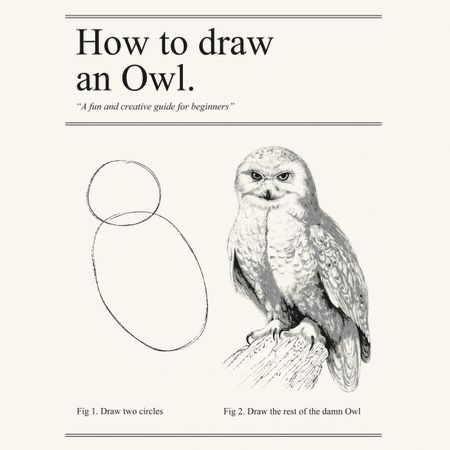
\includegraphics[width=0.5\textwidth]{images/rest-of-the-owl.png}
%   \caption{Two synthesisers on a table, 2019.}
%   \Description{Enjoying looking at two synthesisers.
%   A Korg Monotron and a Korg Volca FM.}
%   \label{fig:teaser}
% \end{teaserfigure}
%%
%% This command processes the author and affiliation and title
%% information and builds the first part of the formatted document.
\maketitle

%%------------------------------------------------------------------------------------------------
% \section*{Remove Me when finished}
% Overleaf seems to break without some text before \verb|\section{Introduction}

Over the past few decades there has been a growing academic movement for an `open methodology' \cite{nosek_scientific_2012}, findable, accessible, interoperable, reproducible (FAIR), and sustainable digital research \cite{go_fair_2016}.
Open and FAIR research practice is vital to ensure transparency, validation, re-use and access within academic research.
The movement has led to an increased awareness across the research community and the establishment of accepted best-practice frameworks \cite{smith_software_2016}. The focus of these frameworks has predominantly been towards digital research practice in the sciences \cite{unesco_open_2021}.


Paper discusses how open research looks at current open research practice at NIME and what could be developed in order to engage wider communities.

\section{Open Research at NIME}

There has been a concerted effort to address the problem of archiving and open-sourcing of DMI over the past 10 years \cite{mcpherson_nimehub_2016,fiordelmondo_longevity_2024,fiordelmondo_towards_2025}. This is not a challenge constrained to just DMI, but is also being addressed as part of the growing open hardware movement.
Open hardware, like open software, is the provision of making electronics designs accessible allowing fabrication outside of a central manufacturer.
\citet{mcpherson_nimehub_2016} and \citet{calegario_documentation_2021} outline largely the same principles as that of the Open Source Hardware Association in 2013 \cite{oshwa_best_2013}, that  unlike software, open hardware cannot be simply distributed as a licence and set of source files (Figure~\ref{fig:osh-taxonomy}), lest it fall afoul of ``openwashing.'' 
\footnote{when a project  ``is claimed to be open source whereas no intention to publish product-related information is given'' \cite{bonvoisin_source_2017}.}  
That is not to say that projects are forbidden, but this should be a conscious choice made at a project's inception and not one applied at a point in the future when the task of archiving a work becomes too great.

\begin{figure*}
    \centering
    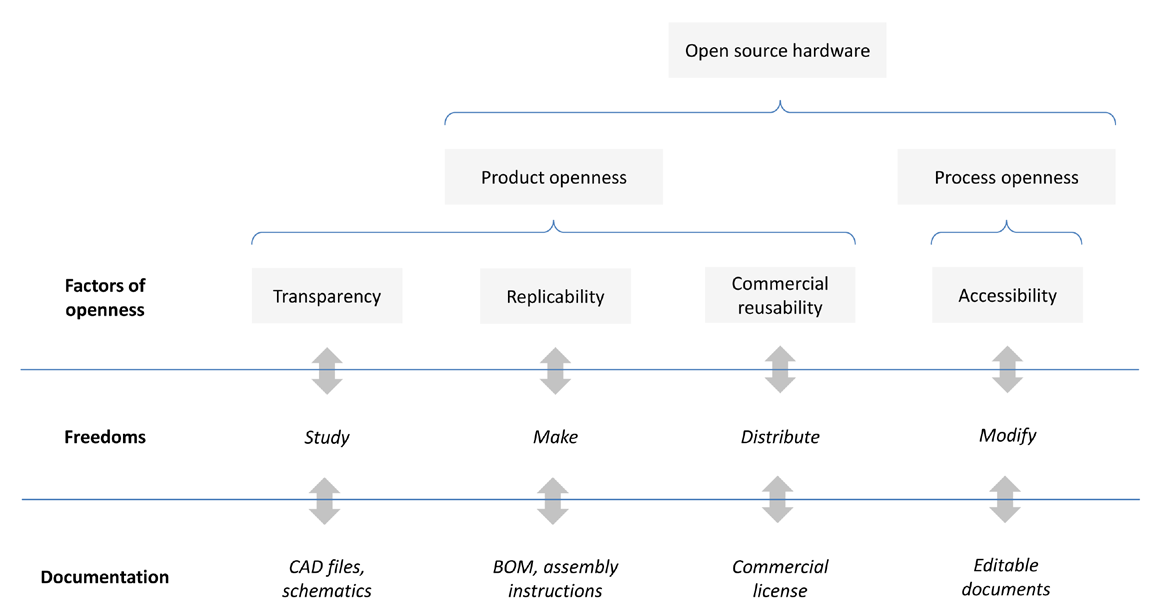
\includegraphics[width=0.9\linewidth]{images/bonvoisin_source_2017-open-hardware.png}
    \caption[Taxonomy of openness]{Taxonomy of openness from \citet[Figure~1]{bonvoisin_source_2017}.}
    \label{fig:osh-taxonomy}
\end{figure*}

\subsection{Previous Work}

Open source hardware has great potential benefits for use in academia \cite{oellermann_open_2022} and those same benefits can extent to the heritage sector. \citet{mcpherson_nimehub_2016} rightfully raises concerns of tackling hardware obsolescence and how that is tackled as part of the archiving process. Proprietary systems limit the potential for innovation or reproducibility and, when these systems fail, repairs rely on the original manufacturer who may have ceased support or production of replacement parts \cite{oellermann_open_2022}.
To facilitate reproduction of hardware, it should be self-evident but, any form of archiving and provision of access to source material makes the task much more feasible. Reproduction is made even easier by incorporating open hardware.
 
An open methodology needs to be `baked-in' to the research process and it is not something trivially applied after the fact. It is of course better to do it afterwards than not at all, but the information at stake also constitutes the development process, not just the end product. The point at which a project is abandoned is not the key point of record.

Both \citet{mcpherson_nimehub_2016} and \citet{fiordelmondo_towards_2025} approach hardware archiving in a repository format. \citet{mcpherson_nimehub_2016} proposed a workshop with the intention to create a a central repository (or database) for DMI designs. Part of that workshop's primary eight goals were the FAIR adjacent aims of encouraging reproducibility, open access and encouraging a normalised practice of documentation. Both \citet{mcpherson_nimehub_2016} and \cite{fiordelmondo_towards_2025} raise the issue of repository structure with the latter proposing a a prescriptive measure which can be applied to any DMI project. Research output in the form of open hardware or open software can and should take advantage of the platforms available for distribution of the work,
\footnote{such as GitHub, GitLab for source code or Thingiverse for 3D models \cite{oshwa_best_2013}.}
but the work still needs to be citable \cite{smith_software_2016}, and cross-reference-able \cite{stall_journal_2023} if it is to be built upon.

The limitation here is assuming that the constituent parts of a DMI are a collective to archive and version controlled. This is true to some degree, there is a complete artefact to be documented, but it is very much made of constituent parts that develop and are swapped out. There is the interface, the electronics, and the firmware, whose versions current and old can be used in all number of combinations of versions. Keeping these components contained to a single version control repository limits their modularity and potential for reuse.


workshops looking at Open NIME research:

\begin{enumerate}
\item \citet{mcpherson_nimehub_2016}
\item \citet{jensenius_open_2019}
\item \citet{jensenius_nime_2020}
\end{enumerate}

% \citet{vallis_shift_2010}

looking at longevity of research \citet{fiordelmondo_longevity_2024}
replicability \cite{calegario_documentation_2021}

work replicating previous NIME's \cite{west_towards_2025}



Review A  of \cite{fiordelmondo_longevity_2024} shows usage of keywords related to version control repositories. 
Review B explores the repositories pertinent to the project being discussed.

projects may cite a github repository but that does not mean the project itself is readily available. The fact it is not immediately apparent the open source nature of project is something that should be addressed.

NIME has had a dedication to making its proceedings publicly available (under a CC by 4.0) from its very inception

as remarked in \citet{calegario_documentation_2021} one can follow the path of \cite{ajin_rebuilding_2019} who created the sponge, and if your lucky, you may even find the original source \url{https://github.com/marierm/sponge-general}.

The recreation of a NIME has focussed on goal of using it musical practice \cite{ajin_rebuilding_2019, masu_nime_2023, west_towards_2025}. Equally valid is the recreation of a NIME for knowledge and development of craft \cite{calegario_documentation_2021}


\subsection{Current State of Open DMIs}\label{sec:current-state}

While instructing university students, the NIME archive has offered a valuable resource for creative applications on the use of micro-controllers, electronics and computer programming. NIME has 2000+ projects available in its open-access archive from which students can draw inspirations and iterate upon. Though many of the projects are open source, far too often this is only on condition that the source can be located in the first place. This raised two questions, the first of which was ``For all papers in NIME, for how many can the source be navigated to from the paper directly?''


\subsubsection{Question 1: Navigating to Source}
To answer the question, the scope of the search was limited to papers from NIME 2025 on which a keyword search was carried out.
Open source research practice has changed since 2001 and the guidance for best-practice academia has developed, from the recommendations in academic open science \cite{go_fair_2016,unesco_open_2021}, open hardware \cite{oshwa_best_2013} and more specifically open research practice at NIME \cite{mcpherson_nimehub_2016,jensenius_open_2019,fiordelmondo_longevity_2024}.
NIME 2025 should therefore represent the `bleeding edge' of open research practice as it will has been informed from guidance available up until this point.

The method used by \citet{calegario_documentation_2021} and Review B from \citet{fiordelmondo_longevity_2024} were used as a starting point for the search. 
Keywords searched included a wildcard ``git*'' (to flag variants such as GitHub and GitLab) as well as
``source,'' ``code,'' and ``doi''.  Upon failing to find any result, the paper was manually skim read to identify alternate methods of including a reference to a source repository.
When a link to source material was found, the URL was recorded alongside the context in which it appeared as well as the page number.

The sum total 96 of papers from 2025 was small enough that a semi-manual approach was achievable in just over three hours. 
% Deriving the context of the URLs would also be much more involved when analysing the the PDF files. 
The rule for what qualified was not whether the source is buildable / executable or even complete, but rather there was a clear intention from the author(s) to make the core source of the project open.
The search aimed to be as forgiving as possible and any completely automated search would like miss instances where the source URLs were not immediately apparent \citet{nime2025_21,nime2025_32}.

Papers with no direct hyperlink, but that included a URL from which the source could be obtained qualified \cite{nime2025_10,nime2025_16,nime2025_21,nime2025_37,nime2025_67}.
Cases where the hyperlink was broken in the PDF but could be easily ascertained and written manually qualified \cite{nime2025_58, nime2025_62}.
\footnote{\citet{nime2025_58} has a space in its source URL and \cite{nime2025_62} has missing underscores, \url{https://github.com/MetaBow/MetaBoard} instead of  \url{https://github.com/MetaBow/_MetaBoard_} }

There were five instances where the link to the repository were unreachable, either requiring authentication or a private repository, or the repository was completely empty. 
The authors were contacted and four out of five have provided an alternative at time of writing.
These repositories are counted, but the recommendations for avoiding such occurrences are covered in Section~\ref{sec:recommendations}.

Of the 96 papers from NIME 2025, there are a total of 34 (\~35\%) that have a clear intention of sharing source, be it software, datasets or even zines\citet{nime2025_42}. This is in keeping with the 33\% reported in \citet{calegario_documentation_2021} which applied a similar process to papers from 2018--2020.
Overwhelmingly GitHub as the preferred platform with 30 projects hosting a repository there, which was the trend identified in \citet{fiordelmondo_towards_2025}. 
Of the 34 papers only one provided a citable digital archive with a DOI \cite{studley_swimtunes_2025}.


\begin{table}
    \centering
    \begin{tabular}{r|cccc}
        \textbf{Placement} & Footnote & Body & Citation & Appendix \\ \hline
        \textbf{\# Papers} & 21       & 8    & 2        & 3        \\
    \end{tabular}
    \caption{Methods for disseminating source URL in NIME 2025 papers.}
    \label{tab:git_placement}
\end{table}


Table~\ref{tab:git_placement} shows how authors from NIME 2025 chose to disseminate source URLs and by far the  most common is a URL in a footnote. Broken down further, 7 papers provided a URL in footnote on the first page an remaining 11 on a later page.

\subsubsection{Question 2: Adoption of Open Source}

The second question was based on analysis by \citet{fiordelmondo_towards_2025} which showed the occurrence of terms related to open source repositories, such as ``git'' and ``repository.''

% Since the search was based on occurrence, it could be skewed by individual with prolific use or citation of open source repositories. 

An individual author / project may employ prolific use of repositories, which would skew the data. Although \citet{fiordelmondo_towards_2025} shows a clear trend towards the adoption of git, a second search was carried out to find to what degree there is a familiarity with git version control we should instead look at in how many papers a git repository is referenced across each year.
 
% What is important is perhaps not the number of occurrences, but whether a paper has relied on the technology at all. 

The PDFs from NIME proceedings were downloaded and separated into directories by year.
Each directory was search for files in which there was an occurrence of git repository. Using the \texttt{pdfgrep} software \cite{deifel_pdfgrep_2024}, papers were searching case-insensitive regular expression \texttt{\\Wgit},
which would capture `git' and variants like `\textbf{Git}Hub' and `\textbf{Git}Lab' but also URLs  like \texttt{https:/\textbf{/git}lab.com/}  or \texttt{oeyvind\textbf{.git}hub.io}.
The list of papers were in which there was a match was counted for each year and shown in Table~\ref{tab:git_occurences}.

in them though 50 papers make reference to `git,' `github,' or `gitlab.'  

The use of git in 50+ papers out the 96 demonstrates a familiarity. 

\begin{table}
    \centering
    \begin{tabular}{r|cccccccccc}
        \textbf{Year}      & \textit{16} & \textit{17} & \textit{18} & \textit{19} & \textit{20} & \textit{21} & \textit{22} & \textit{23} & \textit{24} & \textit{25} \\ \hline
        \textbf{\# Papers} & 16   & 25   & 24   & 29   & 29   & 33   & 24   & 54   & 42   & 50   \\ \hline
        \textbf{\% Overall}& 18   & 24   & 26   & 32   & 29   & 38   & 43   & 54   & 44   & 50   \\ 
    \end{tabular}
    \caption{Number of NIME papers which referenced at least one git repository over the last 10 years. The percentage of papers overall is rounded to the nearest integer.}
    \label{tab:git_occurences}
\end{table}

The number of NIME papers referencing a git repository is broken down in Table~\ref{tab:git_occurences}, for the last 10 years. 

This approach is not fool-proof and misses instance such as \citet{carter_sculpting_2025} where a GitHub repository is available, but it is the url nor the term `git' is reference directly in the text. The result demonstrate a rough trend of increasing familiarity, though over the last few years.

% \cite{fiordelmondo_towards_2025}
% \begin{quote}
%     To contextualise the “github” keyword, we excluded the links referring to GitHub’s web pages, usually in the form \url{https://username.github.io}
% \end{quote}

A deviation from \cite{fiordelmondo_towards_2025} was to not exclude \texttt{github.io} webpages as these results would still suggest usage or some familiarity with GitHub and git software.

Search should be the sum of columns in Table~1 of \citet{fiordelmondo_towards_2025}, but search was not able to produce results nearly as high. A manual search was undertaken to confirm, unless there were searches conducted with information outside the paper, there is no information that would suggest the usage count was as hi as they are for 2022 and 2023

% Have not confirmed with 2024

% \textit{Two Sonification Methods for the MindCube} but \url{https://github.com/mitmedialab/mindcube-rave} is empty except a README

% as does \textit{The Drum Machine of Tao}

%% Sentiment: That for the vast majority of papers, there will be something, and no matter how insignificant or messy, it may provide useful for future understanding
%% 100% adoption is unrealstic, 34% is too low. 

 
The contents and structure of a project repository are flexible, and there is little value in being overly prescriptive, especially given the diversity of papers submitted to NIME. Nevertheless, in the vast majority of cases, a paper can benefit the reader’s understanding through the inclusion of some form of digital material. 
In the course of creating a paper for NIME, which leans so heavily into digital technology there will inevitably in the course of creation be by product, things that made not specifically for the purpose of documentation but made just as part of the process. 

A CAD file for a laser cut enclosure, or PCB, the anonymised results from a user evaluation in a csv file, the python script for generating a plot, the data used to create that plot, the regular expressions used analyse a body of text. The list can go on.

%% Tacit Knowledge
% \cite{schindler_expertise_2015} 
% ``tacit knowledge is assumed to be represented in routinized practices, which are carried
% out in a non-articulate manner (Sennett, 2008, p. 50).''
% papers are explicit knowledge, but can be an answer without the question, a question that might only be illicited from the source material.

Digital research products — the datasets, source code, design files and other artifacts often treated as disposable by researchers — are actually essential for understanding how a project was built and why key decisions were made. These research products will have encoded within the tacit knowledge of engineering practice \citet{schindler_expertise_2015} that are rarely documented but valuable for skill acquisition and future understanding.


\begin{quote}
    Authors cannot identify and report every detail that may be important in a method, but many more parts of the methodology can be shared outside of the report itself.
\end{quote}

\citet{nosek_scientific_2012}. We already do this with video, but the 

% \citet{burns_document_2021}
% \begin{quote}
%     Although this has long been true, the expectations for
% documentation, from the document, have only increased. In the past, when science was offline, it
% was perhaps sufficient to publish a report of an experiment or a study, but now there is a growing
% expectation, and a growing industry, to publish a reproducible work flow, to make the research
% (or lab) notes, software code and scripts, data and and other items publicly available and thus
% depict in the documentation the know-how process of knowledge production.26 This has likewise
% added a burden on the scientist as well as on the infrastructure that supports scientific
% communication, like libraries.
% \end{quote}

A traditional paper alone is often a limited means of describing a Digital Musical Interface and accompanying data, source code, or CAD files are essential to a deeper understanding. Th next section looks at the open methodology through the process of documenting a recent NIME, its limitations and what has been developed since the submission.

\section{An Open Methodology for DMIs}

At nemus realised limitation, keyboard \citet{hamilton_augmentation_2025_activities} had progressed, old links no longer pointed to the keyboard structure of project changing,  two distinct application, one for the museum an another of future research. Bu both used mostly same material. Version tagging helped but how to reference for a paper that would not be misleading. A digital archive of the sing meta solves citation a reference to repo solves outdated links as the metas repo contains submodules. The links for nine 2025 now no longer accurately reflect the state of the keyboard at that time.

Parallel to the physical design, attention was given to documentation and dissemination. Following DMI documentation guidelines \cite{calegario_documentation_2021} and open-science practice \cite{stall_journal_2023}, the entire project was archived: source code, firmware, bill of materials, CAD schematics, STL models, photographs, and build instructions were placed in public repositories. The material is organised into three submodules---\emph{Firmware} \cite{hamilton_firmware_2025}, \emph{CAD} \cite{hamilton_cad_2025}, and \emph{Model Data} \cite{hamilton_models_2025}---combined via a meta-repository (Figure~\ref{fig:repo-relation}). This structure allows individual components (e.g., a PCB or an optical sensor) to be reused or substituted without restructuring the entire system.

\subsection{Modular Source}

Git repo with a single commit hosting static files is no better than serving through a website link to a zip file or a cloud storage (e.g. google drive) link. It does provide potential for greater utility with issues that are tied to the work.

Since Submodules are just a reference to a commit to another repository, the data weight is far smaller than if large sweeping changes in source code or dependencies were stored in the git commit history. There is no requirement for the repositories to share the same platform, and reference will function so long as the upstream repository is accessible.

Such an approach aligns closely with the FAIR principles as it promotes code reuse, interoperability, as well as seamless attribution.

both \citet{calegario_documentation_2021} and \citet{fiordelmondo_longevity_2024} present the idea of a single, unified repository containing all elements. 
Elements such as library dependencies may not be from the original author and other parts may be repurposed from existing projects.
Each element of a DMI may change and to facilitate development and reproducibility a more modular approach is proposed.

Modular source code is aided by the git version control software through its submodules functionality \citet{git_submodule_2025}.

relates to dependencies, but the specific instance where a dependency is one created from the same author(s) or another project that is open source

can describe the project in terms of parts that may be swapped. The burden of redundant replication is lifted, without sacrificing the traceability.

The aim is not to be reductionist ``by lieu of ... components'' \cite{burns_documents_2021}, quite the opposite, that sokething can be more than the some of its parts.

\subsection{Version Control}

The interface project highlighted limitations within the archiving frameworks that are currently available. A benefit of the Zenodo archive is its integration to GitHub. This allows a single project to be simultaneously maintained and archived for citation from a single location.
Unfortunately, the GitHub integration for Zenodo does not currently provide a means for meta-repositories to be archived correctly \cite{zenodo_1036_2025}. This limitation necessitates the generation of a separate DOI for each component submodule, all of which reference the meta-repository.

\begin{figure}
\centering
    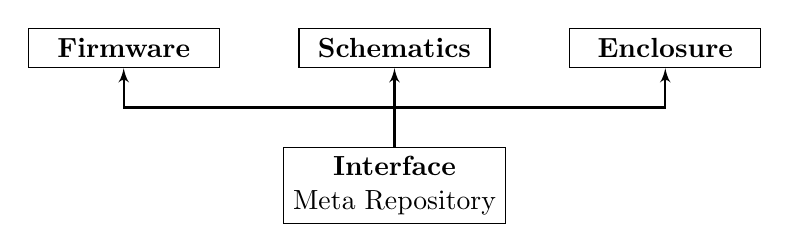
\begin{tikzpicture}[
      box/.style = {draw, minimum width=0.2\linewidth, minimum height=0.5cm, align=center},
      arrow/.style = {-latex', thick}
    ]
    
    % \node[box] (box1) {Firmware\\sub-module};
    % \node[box, right=of box1] (box2) {CAD\\sub-module};
    % \node[box, right=of box2] (box3) {Model Data\\sub-module};
    % \node[box, below=2cm of box2] (bottom) {Interface\\meta-repository};

    \node[box] (box1) {\textbf{Firmware}};
    \node[box, right=of box1] (box2) {\textbf{Schematics}};
    \node[box, right=of box2] (box3) {\textbf{Enclosure}};
    \node[box, below=1cm of box2] (bottom) {\textbf{Interface}\\Meta Repository};
    
    \draw[arrow] (bottom.north) -- ++(0,0.5) -| (box1.south);
    \draw[arrow] (bottom.north) -- ++(0,0.5) -| (box2.south);
    \draw[arrow] (bottom.north) -- ++(0,0.5) -| (box3.south);
    
    \end{tikzpicture}
    \caption{The DMI is divided into three submodules each representing the firmware, electronics schematics and enlosure modelling data. These submodules are collected into a single repository that represents the interface.}
    \label{fig:repo-relation}
\end{figure}

\subsection{Archiving}

Archiving provides a means by which a work can be cited.

A DMI as a research product \cite{xxx} is an object that should be citable. The paper describes the object, it is not object itself and there are instances where citing the object is more applicable than citing the paper based around it.

Archiving should provide a DOI with which to cite. Repositories may also provide a recommended citation, but this should very much be looked upon as a bandage to a broken system and not a solution. The very helpful citation file format CFF provides a means to have a structure citation to software, but unhelpfully, integration with GitHub prompts the user to ``Cite this Repository'' \url{https://docs.github.com/en/repositories/managing-your-repositorys-settings-and-features/customizing-your-repository/about-citation-files} which, as already discussed, is something to be avoided.

Archiving exposed a few practical challenges. Zenodo’s GitHub integration does not yet handle meta-repositories, requiring separate DOIs for each submodule with cross-references \cite{zenodo_1036_2025}. Likewise, the future of CAD data is tied to software sustainability: the discontinuation of Autodesk EAGLE \cite{autodesk_eagle_2024} effectively freezes its XML format, though conversion to KiCad remains available \cite{kicad_eagle_2024}. These lessons emphasise that openness depends not only on licensing but also on the careful selection of formats and hosting infrastructure.

\begin{figure}
    \centering
    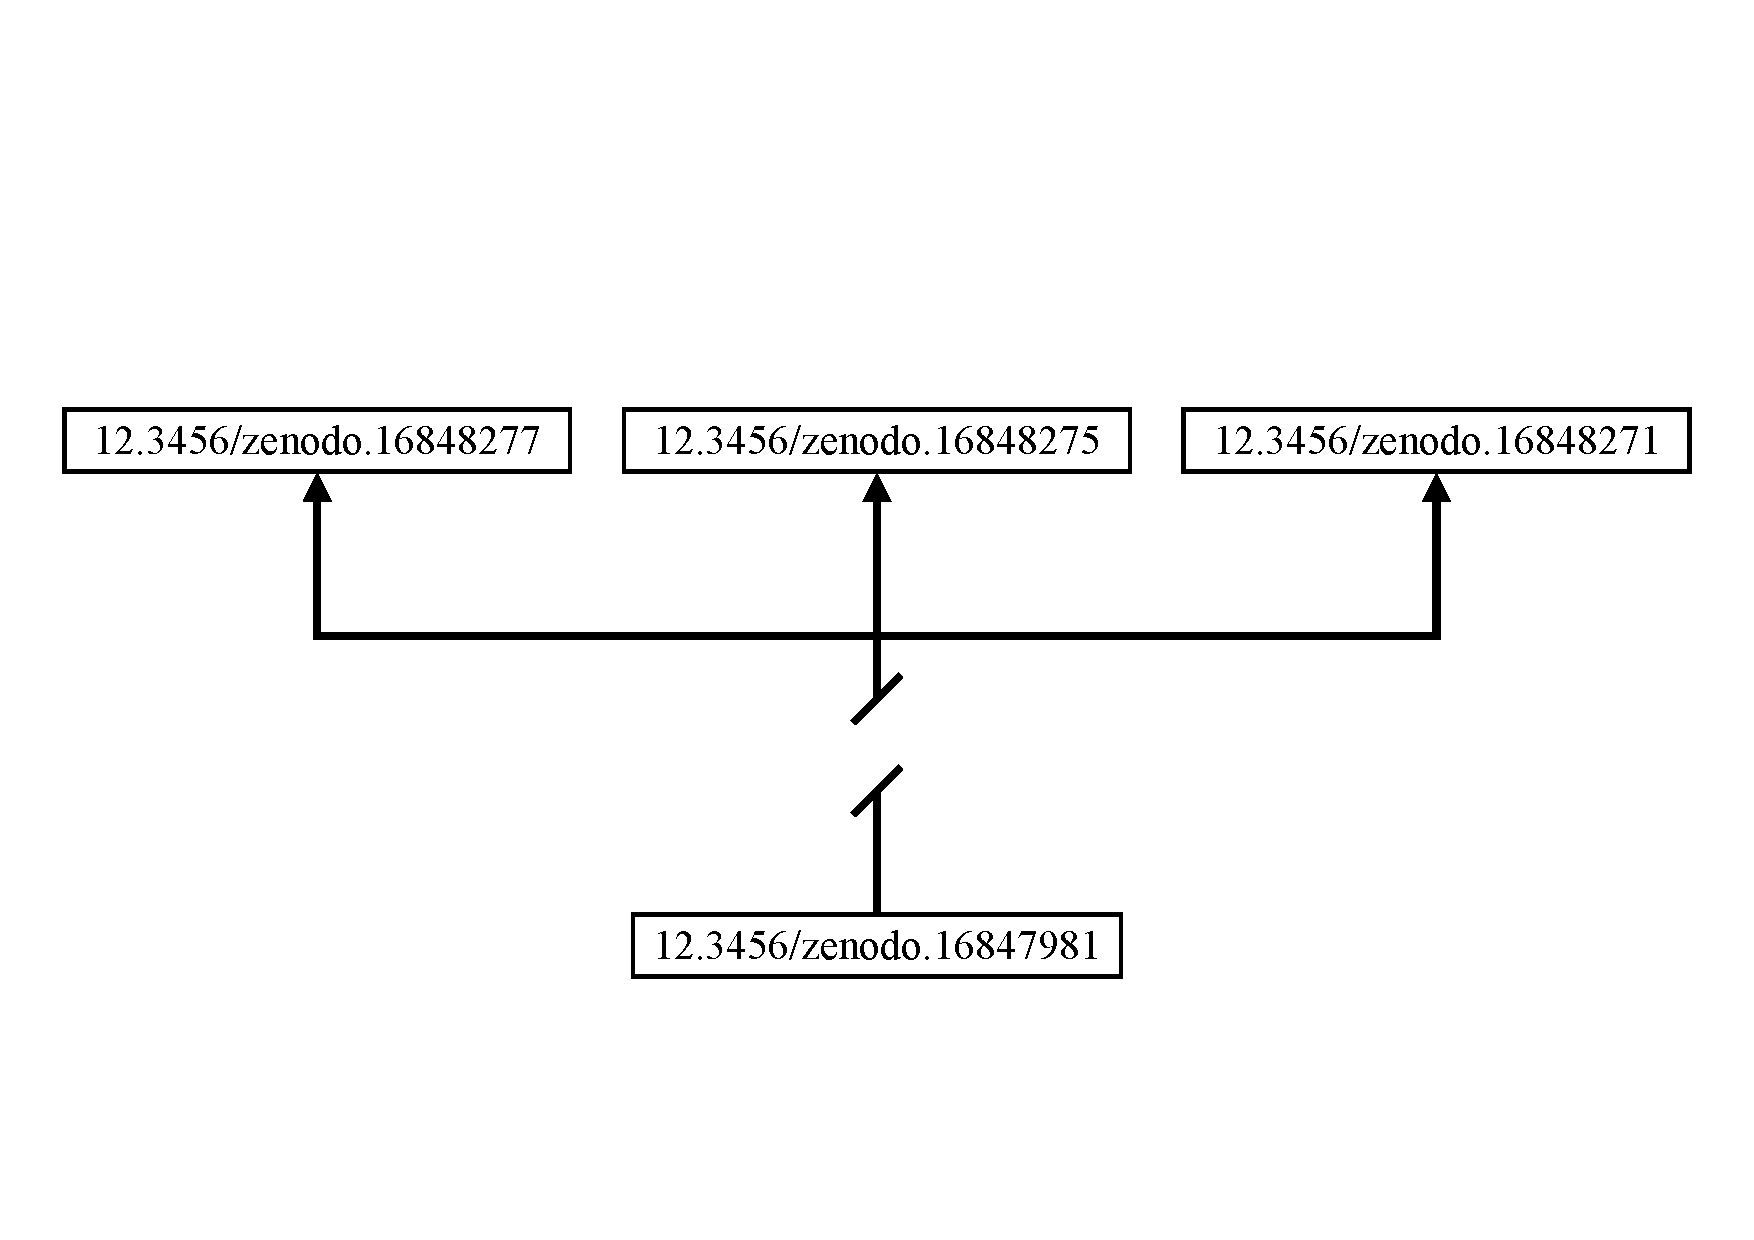
\includegraphics[width=1\linewidth]{images/modular_archive_1.pdf}
    \caption{Zenodo's GitHub integration does not include data in submodules. Alternative process is to archive each submodule at the relevant version and then archive the meta repository which contains the separate DOIs.}
    \label{fig:zenodo-github-integration}
\end{figure}

\subsubsection{limits in archiving modular projects}

Problem with a modular process is that zenodo's integration does not support it or a allow for easy configuration.

Would require the manual creation of the archive, copy the contents over. Alternatively, each submodule could be archived and a meta-archive simply contains reference to the constituent DOIs. This is not ideal but it is also not insurmaountable.



\subsection{Version Control $\neq$ Archiving}

a version control repository is not an archive.

longevity of a version control repository should be treated cautiously especially when it is privately owned. institutes could do more to provide these kind of services, but that is a separate discussion.

Version control allows a project to be explored in time. The version pertaining to the project should be tagged, of course, but a version control repository is a living document.

The content of a version control repository is alive and its location is ephemeral. A digital archive's content is static and location permanent.

Version control repository ideal for idea that iterate and where there is a desire to navigate a project's progression in time.

For citing work, given their static and permanent nature, archives and DOIs should be used.

\subsection{Documentation}

Following \citet{procida_diataxis_2025}, four complementary forms of
documentation can be distinguished: Tutorials, How-to guides, Explanation, and
Reference. These forms naturally divide into two audiences: user-facing and
developer-facing. Adapting \citet{procida_diataxis_2025}, developer-facing
documentation lies in the How-to and Reference categories, while user-facing
documentation is found in Tutorials and Explanation. This division is not
strict, as the binary of `user' and `developer' rarely holds true in practice;
rather, audiences exist along a continuum. Reference documentation can be
generated from source annotations to avoid duplication and support automation.
Across M\textsc{atlab}, Python, and C\textsc{++}, multiple conventions coexist
\cite{vanrossum_pep8_2001, goodger_pep257_2001}, supported by tooling ecosystems
such as Doxygen, Sphinx, and HeaderDoc.%
\footnote{See the Stack Overflow Data Explorer for indicative tag counts:
\url{https://data.stackexchange.com/stackoverflow/query/1069131/get-all-tags}.}
Even so, generated API references should not substitute for user manuals
\cite[Section~6.2]{stallman_gnu_1992}, though this is often the case
\cite{procida_diataxis_2025}.%
\footnote{\url{https://diataxis.fr/reference/}}

Best practice emphasises the importance of documentation
\cite{smith_software_2016}, though it is less prescriptive about form and depth.
\citet{writethedocs_sowftware_2025} offers comprehensive guidance; a
pragmatic rule is that documentation should enable you to still ``understand
your code in six months'' \cite{writethedocs_sowftware_2025}, a principle echoed
in reproducibility studies \cite{perkel_challenge_2020}. Using the
\citep{ssi_checklist_2018} checklist, the core requirements for an open research
software project are: publicly available source code, a version control system
(VCS), user and developer documentation, an OSI-compliant licence, and
persistent identifiers (typically DOIs). A public VCS implies source
availability, though the reverse is not guaranteed. Likewise, a DOI implies some
level of digital archiving, but a release archive does not necessitate a DOI.
DOIs should be assigned both to the software as a whole and to individual
releases \cite{smith_software_2016}; licences should be clearly stated and
OSI-compliant \cite{hong_choosing_2025}. To better support complex software
citation, \citet{druskat_citation_2021} introduced the Citation File Format
(CFF), which standardises metadata for software citations and is supported by
both GitHub and Zenodo. Recommendations in \citet{fiordelmondo_towards_2025}
extend this to hardware projects, with tools for citation
\cite{spaaks_cffconvert_2021}. Beyond these essentials (contribution policies,
issue tracking, codes of conduct), more advanced practices presuppose an active
repository.

Shallow submodules allow for only the relevant code for that commit to be pulled from the upstream repository meaning the full data weight of the entire repository is not needed.
Relevant for the ability to compartmentalise auto generated documentation which can be served from a sub-repository branch, but not clog up the  code base of the meta repository.
This was the case with the firmware \footnote{\url{https://nemus-project.github.io/harpsichord-interface-firmware/docs/html/}} for interface in \citet{hamilton_augmentation_2025_activities}.


\subsubsection{Software Documentation Practice}

The documentation practice for a project may also reveal something within the author's own perception of the work.
Documentation that leans heavily towards \textit{Reference} in the diataxis framework \citet{procida_diataxis_2025} are concerned with the technical understanding and modification of the work, something that is still in progress.
In the same framework, ``Tutorial'' documentation view the work is static, when the user's primary concern is with utilising the work. Through this lens we can assess a NIME and perhaps understand the intention for growth or reuse.

% \cite{burns_documents_2021}
% \begin{quote}
%     Case in point: I highly doubt anyone
% has learned to ride a bike by reading an instruction manual.
% \end{quote}
%  But somone needed to explain it


\section{Concluding Remarks}

Reluctance to share, anecdotally is that a work is `in-progress' which should be seen as a benefit. The appearance that work is in a highly finished polished state can be intimidating. the goal of NIME is should not always be to have a completed idea but to discuss ideas in progress. If that were the case we would \textit{only} be sharing pictures and archives, once something is finished, what isthere kef6t to discuss.

Designing Sensory NIME for Autism: ``Open-source development initiatives should be encouraged to foster 
scalability and inclusivity.''


Sharing with a wider community enables the possibility of research breaking out beyond the confines of its original life span. Enables the chance for more meaningful user evaluation \cite{calegario_documentation_2021} by reducing the barriers to accessing an interface. Ideas can be iterated upon, built upon previous work.

Source material varies from schematics to zine \cite{nime2025_42}.

% \citet{burns_documents_2021}
% \begin{quote}
%     Thus, even though the administration would agree
% that the library was a real place, it was only real to them as the “cobblestones” of the street are
% real—as opposed to whole streets with their social worlds and other components (the whole is
% reduced to a part that then becomes its perceived entire ontological substance; perhaps we can
% think of this as synecdochic fallacy38). However, per Polanyi, this is a failure to recognize
% emergence:
% This capacity of a thing to reveal itself in unexpected ways in the future I attribute to the
% fact that the thing observed is an aspect of a reality, possessing a significance that is not
% 14
% exhausted by our conception of any single aspect of it…. And since I regard the
% significance of a thing as more important than its tangibility, I shall say that minds and
% problems are more real than cobblestones.39
% If we can apply this lesson to the document, we could state that:
% Thesis 5: Tacit knowledge warns us against treating the digital document as if it is only a
% cobblestone.
% Yet this is what the open science movement does, not by introducing a new paradigm but
% by expanding the task assigned to the document—to document more, for example, under the
% FAIR principle (findable, accessible, interoperable, reusable).40
% \end{quote}

% Yet this is what the open science movement does, not by introducing a new paradigm but
% by expanding the task assigned to the document—to document more, for example, under the
% FAIR principle (findable, accessible, interoperable, reusable).40 
% Not to document more for the sake of documentation but to share and make open what is already there and what might already be being shared and open, but just done in a deliberate manner.
% work reduced to a cobblestone, be delibarate


% \subsection{Core principles}

% 1. It should be easy to find a repository (version control or archival)
% 2. if it exists, it should be in the paper
% 3. open should be the default
% 4.


\section{Recommendations}\label{sec:recommendations}

What the repository or archive of the DMI should contain has already been covered elsewhere, the specific contents are not fixed and will change from project to project

rather than focussing on a central repository \citet{mcpherson_nimehub_2016}, electing replicating officers \citet{calegario_documentation_2021} or conforming to standard format \citet{fiordelmondo_towards_2025} we can look at solution that are much simpler, but have a much wider impact

clear there is a desire to share work, offload the burden on choosing the most effective way to disseminate, or the reader in locating the work, the solution would be to standardise one, possibly two field that are in the papers template text, and in the metadata.

The burden to choose a format on the author and burden of finding it on the reader as opposed to an agreed format understood by both parties.


Table~\ref{tab:git_placement}
This is not a call to conform to this as standard practice, but the variation in placement shows there is no universal strategy by which the community has aligned. 
A suggested solution to address this is covered in section \ref{sec:recommendations}.


Section~\ref{sec:current-state}
In most cases there was a clear desire to make the work accessible, but with no clear format the link was overlooked.
Two repositories were private and subsequently made available, one repository had simply used the wrong link and alternate was provided.
For one repository, the authors were unreachable. Finally, one repository was found through a simple search. Including these papers which had intent, the total is 34 repositories.

\footnote{Or examples such as \textit{Embedded Comparo: Small DSP Systems Side-by-Side} where the git repository url is easily missed as a footnote hidden below references.}

The infrastructure exists \url{https://arxiv.org/} and \url{https://zenodo.org/} are openly available and relevant, withthe latter the standard archive for NIME proceedings.
\footnote{with the exception of 2022 and 2023 which use pubpub \url{https://nime.pubpub.org/previous-nimes}}
Part of the submission, the work can marked as closed source, if that is necessary but a mandatory field for project URL or DOI would curtail the open source agnosticism and make the choice a much more deliberate one.

NIME already provides a an entry in its metadata for an archive from which the paper's DOI is taken. Of the 96 NIME 2025 papers only 16 papers have supplementary files and these are exclusively videos.
When source material is extant and there is a clear intention on sharing it, it would appear that some barrier is present which prevents or dissuades authors from sharing their supplementary material.

\begin{figure}
    \centering
    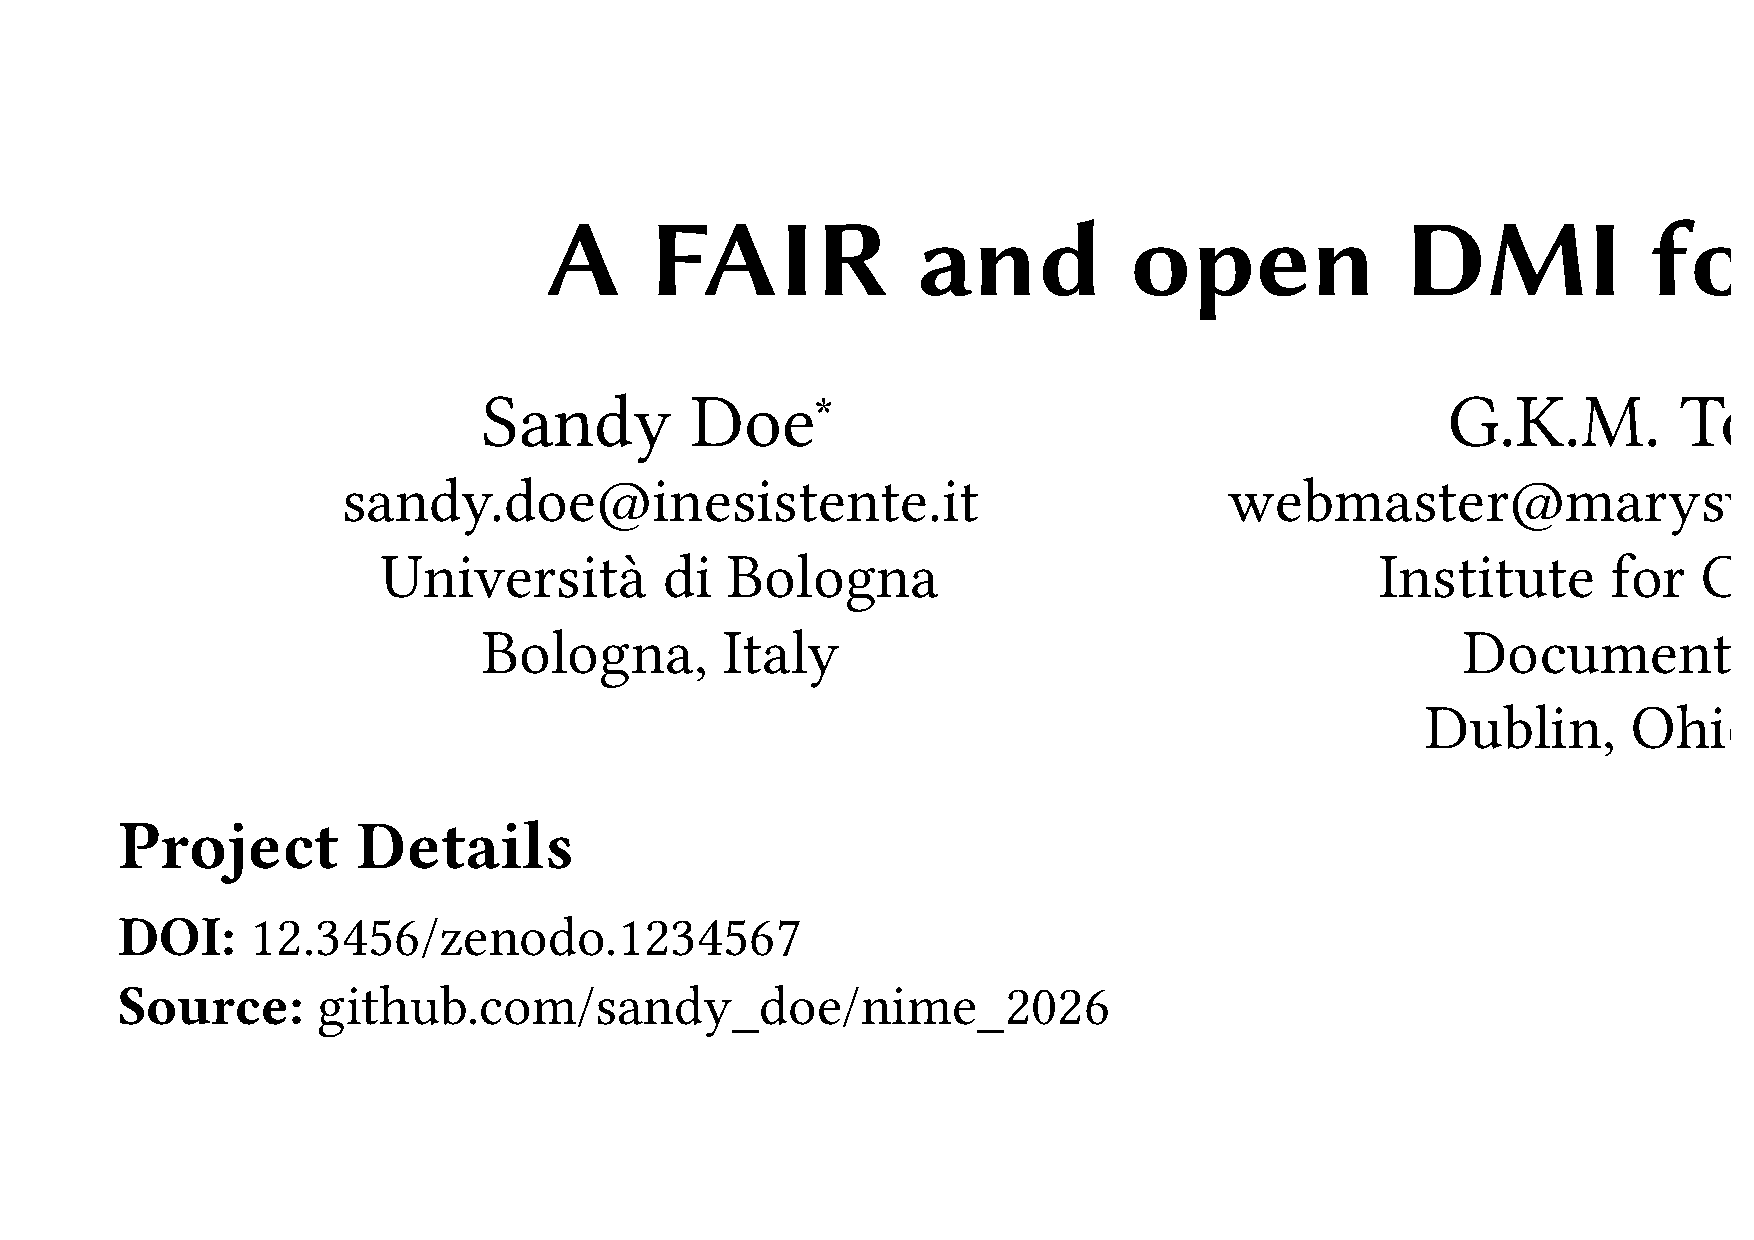
\includegraphics[width=\linewidth]{images/open-example.pdf}\\
    \vspace{0.5cm}
    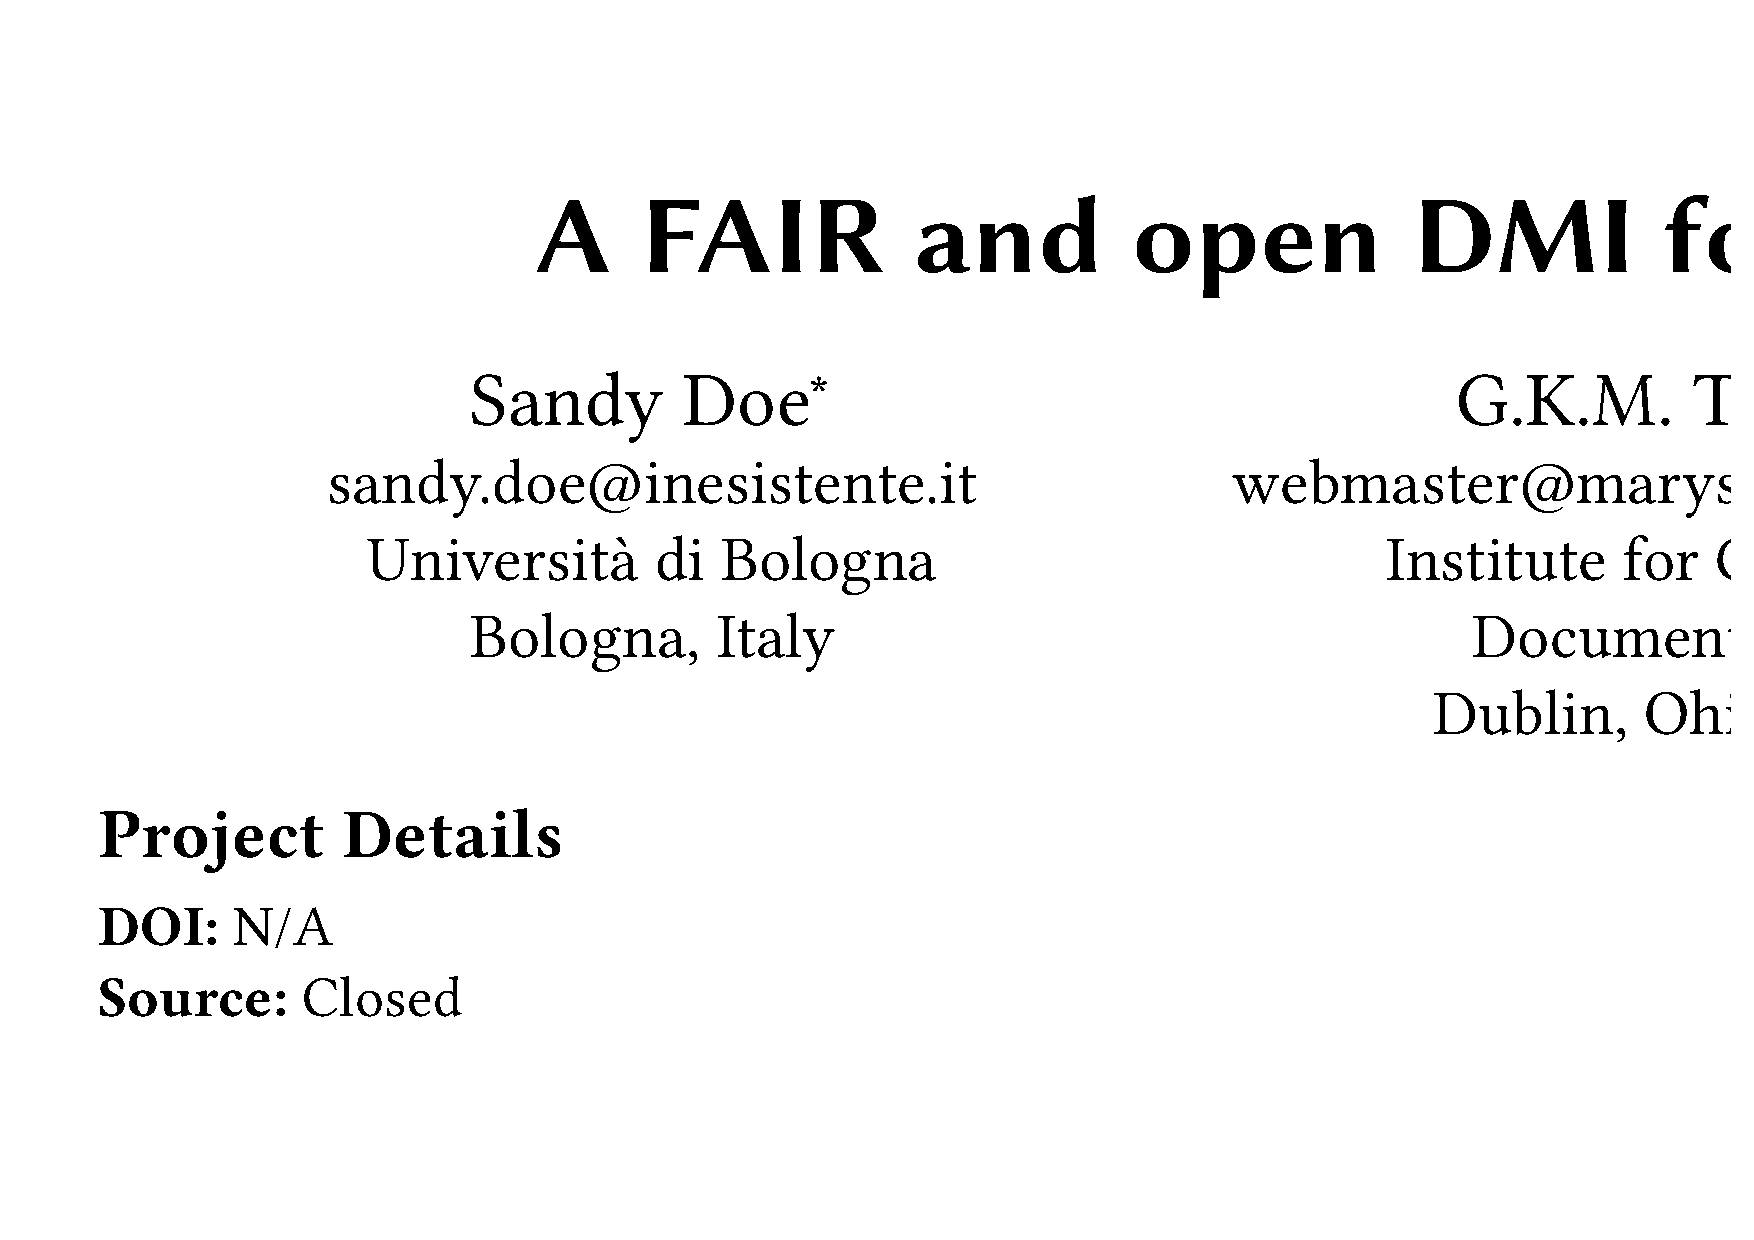
\includegraphics[width=\linewidth]{images/closed-example.pdf}    
    \caption{Project details as a standard field in the paper template, in the same manner of the title and authors, would allow for quick identification of the project status and files. These details are not obligatory and could be withheld, but the choice to do so becomes deliberate.}
    \label{fig:project-details}
\end{figure}

Aiming for some standardised template or central repository sets a high bar that the community is npt ready to meet. We may be missing even just the obvious solutions.
One can find the authors of a paper easily. Supplementary material in the form of a zenodo archive has a space on the NIME website, but it is clearly under utilised.

In the same way one can open a per and see immediately the title, authors, there should be a space for
a DOI to the source for which the material pertains or a notice in cases where the the work is either proprietary or the material has some other ethical restrictions.

For academic work, an open first approach should be the goal standard as recommended in the open science and FAIR principles. Closed by default because of a clear path to sign-post a repository is a huge waste.

for example: SMucK: Symbolic Music in ChucK is perfectly easy to find with a search, but it is missing any kind of link in the paper! (disqualified)

A standard metadata entry would ease future analysis.


fits in to the wider practice of citing digital research output, be it software, hardware, or data. The process very quickly becomes messy which is more often than not as the ideal is of a standard citation is not available.

This has been the case for this paper, and likely many papers at this years NIME.

% What is a clear order of precedence for citing sowftare?
A clear order of precedence

\begin{itemize}
\item DOI to the archive of the relevant version
\item SoftWare Hash IDentifier (SWHID) \cite{softwareheritage_archive_2025}
\item Citation File Format \cite{druskat_citation_2021}
\item Suggested citation format
\item Version-specific repository URL
\item General project URL
\end{itemize}

When citing software or data, precedence should favour a citation that prioritises longevity and version specificity over those that merely indicate location.

SoftWare Hash IDentifier (SWHID) ISO/IEC international standard 18670 on April 23, 2025.
Is passive, requires the repository be public and cannot guarantee that submodules have also been ingested. 

Like the web archive, this should be looked upon as a last ditch and a much more active and deliberate archiving approach should be taken

%% Sentiment: The intention is end on note that acknowledges that this isn't zero effort, but it is worth while. That nothing will improve if we do nothing. 
%% The sentiment is also that there is an implicit high bar and far to few are meeting it, so we should lower to an _explicit_. 
%% Perfect is the enemy of good, 
%% good-enough practice before best practice
The resistance is very much one of awareness and skill acquisition. Contributors are far more likely to follow the practice set out by there peers and their mentors. Change comes from above, and from the side and we should lead by example.

|. All relevant text is in 
% \texttt{article.tex}

% 
Possible Paper Categories:

4000 words (now “medium”, formerly “short”)

2000 words (now “short”, formerly “demo”)

Structure of the paper:

\section{Introduction}
present the topic and outline the structure of the paper

Including what is FAIR \citet{wilkinson_fair_2016} Open Science \citet{burgelman_open_2019} and how open is not enough \citet{chen_open_2019}.

\section{FAIR, Open Source Digital Musical Interfaces (DMI) at NIME}

Section explores the work that has been done and assessment of 

\subsection{Relevant Work}
Previous papers that have addressed open source hardware and the open sourcing at NIME

Of note:

\begin{enumerate}
    \item  \citet{fiordelmondo_towards_2025}
    \item  \citet{clarke_longevity_2025}
    \item  \citet{calegario_documentation_2021}
    \item  \citet{colazo_licence_2009}
    \item  \citet{perkel_challenge_2020}
    \item  \citet{robert_reproducibility_2020}
    \item  \citet{mcpherson_nimehub_2016}
    \item  \citet{bonvoisin_source_2017}
    \item  \citet{fiordelmondo_longevity_2024}    
\end{enumerate}

\subsection{State of Open Source at NIME 2025}
An audit of NIME 2025 papers and the alignment with FAIR principles.

\section{An Open Methodology for DMIs}
Presentation of an open methodology that can be applied to DMIs using \cite{hamilton_augmentation_2025_activities} as a case study covering the following elements.

\subsection{Source}
Modular source, with though given to dependencies and how parts of the project may be used \textit{outside} of the project itself.
\subsection{Version Control}
A repository to navigate through the evolution of a project.
If a meta repository approach is taken, the meta repository will always be a snapshot, less granular than the individual submodules.
\subsection{Archiving}
The archiving of the project, collecting all elements and assigning a DOI and a space that has longevity. Institutional Archive or independent, like  Zenodo.
\subsection{Version Control $\neq$ Archiving}
A version control repository is not a substitute for an archival repository.

on software and citation

\begin{enumerate}
    \item  \citet{stall_journal_2023}
    \item  \citet{soito_citations_2016}
    \item  \citet{katz_recognizing_2021}
    \item  \citet{smith_software_2016}
\end{enumerate}

\subsection{Documentation}
Diataxis can be used as a framework. The documentation addresses two groups, users and developers. 

\subsection{Licensing}
A suitable open source licence, the choice of which has implication on archiving on platforms like zenodo

\section{Concluding remarks and Recommendations}

If you want to engage with wider communities, reduce the friction for that community to engage with the work.
Readers should not be burdened with detective work and solving the problem of creating a standard disseminating and project source should not be replicate across authors.
Suggested solutions: a field in the metadata and a space in the paper template for 1. the project VCS repository and 2. the project archive.
% A recent report shows a clear digital skill gap in humanities compared to the sciences \cite{taylor_shaping_2022}.
\section{Introduction}

Over the past few decades there has been a growing academic movement for an `open methodology' \cite{nosek_scientific_2012}, findable, accessible, interoperable, reproducible (FAIR), and sustainable digital research \cite{go_fair_2016}.
Open and FAIR research practice is vital to ensure transparency, validation, re-use and access within academic research.
The movement has led to an increased awareness across the research community and the establishment of accepted best-practice frameworks \cite{smith_software_2016}. The focus of these frameworks has predominantly been towards digital research practice in the sciences \cite{unesco_open_2021}.


Paper discusses how open research looks at current open research practice at NIME and what could be developed in order to engage wider communities.

\section{Open Research at NIME}

There has been a concerted effort to address the problem of archiving and open-sourcing of DMI over the past 10 years \cite{mcpherson_nimehub_2016,fiordelmondo_longevity_2024,fiordelmondo_towards_2025}. This is not a challenge constrained to just DMI, but is also being addressed as part of the growing open hardware movement.
Open hardware, like open software, is the provision of making electronics designs accessible allowing fabrication outside of a central manufacturer.
\citet{mcpherson_nimehub_2016} and \citet{calegario_documentation_2021} outline largely the same principles as that of the Open Source Hardware Association in 2013 \cite{oshwa_best_2013}, that  unlike software, open hardware cannot be simply distributed as a licence and set of source files (Figure~\ref{fig:osh-taxonomy}), lest it fall afoul of ``openwashing.'' 
\footnote{when a project  ``is claimed to be open source whereas no intention to publish product-related information is given'' \cite{bonvoisin_source_2017}.}  
That is not to say that projects are forbidden, but this should be a conscious choice made at a project's inception and not one applied at a point in the future when the task of archiving a work becomes too great.

\begin{figure*}
    \centering
    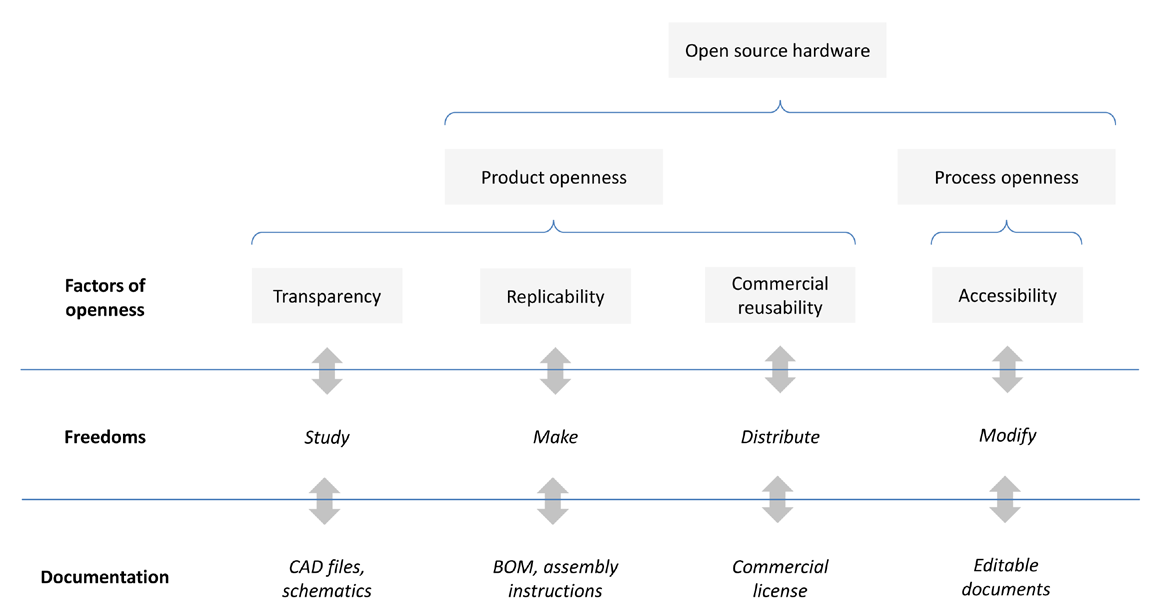
\includegraphics[width=0.9\linewidth]{images/bonvoisin_source_2017-open-hardware.png}
    \caption[Taxonomy of openness]{Taxonomy of openness from \citet[Figure~1]{bonvoisin_source_2017}.}
    \label{fig:osh-taxonomy}
\end{figure*}

\subsection{Previous Work}

Open source hardware has great potential benefits for use in academia \cite{oellermann_open_2022} and those same benefits can extent to the heritage sector. \citet{mcpherson_nimehub_2016} rightfully raises concerns of tackling hardware obsolescence and how that is tackled as part of the archiving process. Proprietary systems limit the potential for innovation or reproducibility and, when these systems fail, repairs rely on the original manufacturer who may have ceased support or production of replacement parts \cite{oellermann_open_2022}.
To facilitate reproduction of hardware, it should be self-evident but, any form of archiving and provision of access to source material makes the task much more feasible. Reproduction is made even easier by incorporating open hardware.
 
An open methodology needs to be `baked-in' to the research process and it is not something trivially applied after the fact. It is of course better to do it afterwards than not at all, but the information at stake also constitutes the development process, not just the end product. The point at which a project is abandoned is not the key point of record.

Both \citet{mcpherson_nimehub_2016} and \citet{fiordelmondo_towards_2025} approach hardware archiving in a repository format. \citet{mcpherson_nimehub_2016} proposed a workshop with the intention to create a a central repository (or database) for DMI designs. Part of that workshop's primary eight goals were the FAIR adjacent aims of encouraging reproducibility, open access and encouraging a normalised practice of documentation. Both \citet{mcpherson_nimehub_2016} and \cite{fiordelmondo_towards_2025} raise the issue of repository structure with the latter proposing a a prescriptive measure which can be applied to any DMI project. Research output in the form of open hardware or open software can and should take advantage of the platforms available for distribution of the work,
\footnote{such as GitHub, GitLab for source code or Thingiverse for 3D models \cite{oshwa_best_2013}.}
but the work still needs to be citable \cite{smith_software_2016}, and cross-reference-able \cite{stall_journal_2023} if it is to be built upon.

The limitation here is assuming that the constituent parts of a DMI are a collective to archive and version controlled. This is true to some degree, there is a complete artefact to be documented, but it is very much made of constituent parts that develop and are swapped out. There is the interface, the electronics, and the firmware, whose versions current and old can be used in all number of combinations of versions. Keeping these components contained to a single version control repository limits their modularity and potential for reuse.


workshops looking at Open NIME research:

\begin{enumerate}
\item \citet{mcpherson_nimehub_2016}
\item \citet{jensenius_open_2019}
\item \citet{jensenius_nime_2020}
\end{enumerate}

% \citet{vallis_shift_2010}

looking at longevity of research \citet{fiordelmondo_longevity_2024}
replicability \cite{calegario_documentation_2021}

work replicating previous NIME's \cite{west_towards_2025}



Review A  of \cite{fiordelmondo_longevity_2024} shows usage of keywords related to version control repositories. 
Review B explores the repositories pertinent to the project being discussed.

projects may cite a github repository but that does not mean the project itself is readily available. The fact it is not immediately apparent the open source nature of project is something that should be addressed.

NIME has had a dedication to making its proceedings publicly available (under a CC by 4.0) from its very inception

as remarked in \citet{calegario_documentation_2021} one can follow the path of \cite{ajin_rebuilding_2019} who created the sponge, and if your lucky, you may even find the original source \url{https://github.com/marierm/sponge-general}.

The recreation of a NIME has focussed on goal of using it musical practice \cite{ajin_rebuilding_2019, masu_nime_2023, west_towards_2025}. Equally valid is the recreation of a NIME for knowledge and development of craft \cite{calegario_documentation_2021}


\subsection{Current State of Open DMIs}\label{sec:current-state}

While instructing university students, the NIME archive has offered a valuable resource for creative applications on the use of micro-controllers, electronics and computer programming. NIME has 2000+ projects available in its open-access archive from which students can draw inspirations and iterate upon. Though many of the projects are open source, far too often this is only on condition that the source can be located in the first place. This raised two questions, the first of which was ``For all papers in NIME, for how many can the source be navigated to from the paper directly?''


\subsubsection{Question 1: Navigating to Source}
To answer the question, the scope of the search was limited to papers from NIME 2025 on which a keyword search was carried out.
Open source research practice has changed since 2001 and the guidance for best-practice academia has developed, from the recommendations in academic open science \cite{go_fair_2016,unesco_open_2021}, open hardware \cite{oshwa_best_2013} and more specifically open research practice at NIME \cite{mcpherson_nimehub_2016,jensenius_open_2019,fiordelmondo_longevity_2024}.
NIME 2025 should therefore represent the `bleeding edge' of open research practice as it will has been informed from guidance available up until this point.

The method used by \citet{calegario_documentation_2021} and Review B from \citet{fiordelmondo_longevity_2024} were used as a starting point for the search. 
Keywords searched included a wildcard ``git*'' (to flag variants such as GitHub and GitLab) as well as
``source,'' ``code,'' and ``doi''.  Upon failing to find any result, the paper was manually skim read to identify alternate methods of including a reference to a source repository.
When a link to source material was found, the URL was recorded alongside the context in which it appeared as well as the page number.

The sum total 96 of papers from 2025 was small enough that a semi-manual approach was achievable in just over three hours. 
% Deriving the context of the URLs would also be much more involved when analysing the the PDF files. 
The rule for what qualified was not whether the source is buildable / executable or even complete, but rather there was a clear intention from the author(s) to make the core source of the project open.
The search aimed to be as forgiving as possible and any completely automated search would like miss instances where the source URLs were not immediately apparent \citet{nime2025_21,nime2025_32}.

Papers with no direct hyperlink, but that included a URL from which the source could be obtained qualified \cite{nime2025_10,nime2025_16,nime2025_21,nime2025_37,nime2025_67}.
Cases where the hyperlink was broken in the PDF but could be easily ascertained and written manually qualified \cite{nime2025_58, nime2025_62}.
\footnote{\citet{nime2025_58} has a space in its source URL and \cite{nime2025_62} has missing underscores, \url{https://github.com/MetaBow/MetaBoard} instead of  \url{https://github.com/MetaBow/_MetaBoard_} }

There were five instances where the link to the repository were unreachable, either requiring authentication or a private repository, or the repository was completely empty. 
The authors were contacted and four out of five have provided an alternative at time of writing.
These repositories are counted, but the recommendations for avoiding such occurrences are covered in Section~\ref{sec:recommendations}.

Of the 96 papers from NIME 2025, there are a total of 34 (\~35\%) that have a clear intention of sharing source, be it software, datasets or even zines\citet{nime2025_42}. This is in keeping with the 33\% reported in \citet{calegario_documentation_2021} which applied a similar process to papers from 2018--2020.
Overwhelmingly GitHub as the preferred platform with 30 projects hosting a repository there, which was the trend identified in \citet{fiordelmondo_towards_2025}. 
Of the 34 papers only one provided a citable digital archive with a DOI \cite{studley_swimtunes_2025}.


\begin{table}
    \centering
    \begin{tabular}{r|cccc}
        \textbf{Placement} & Footnote & Body & Citation & Appendix \\ \hline
        \textbf{\# Papers} & 21       & 8    & 2        & 3        \\
    \end{tabular}
    \caption{Methods for disseminating source URL in NIME 2025 papers.}
    \label{tab:git_placement}
\end{table}


Table~\ref{tab:git_placement} shows how authors from NIME 2025 chose to disseminate source URLs and by far the  most common is a URL in a footnote. Broken down further, 7 papers provided a URL in footnote on the first page an remaining 11 on a later page.

\subsubsection{Question 2: Adoption of Open Source}

The second question was based on analysis by \citet{fiordelmondo_towards_2025} which showed the occurrence of terms related to open source repositories, such as ``git'' and ``repository.''

% Since the search was based on occurrence, it could be skewed by individual with prolific use or citation of open source repositories. 

An individual author / project may employ prolific use of repositories, which would skew the data. Although \citet{fiordelmondo_towards_2025} shows a clear trend towards the adoption of git, a second search was carried out to find to what degree there is a familiarity with git version control we should instead look at in how many papers a git repository is referenced across each year.
 
% What is important is perhaps not the number of occurrences, but whether a paper has relied on the technology at all. 

The PDFs from NIME proceedings were downloaded and separated into directories by year.
Each directory was search for files in which there was an occurrence of git repository. Using the \texttt{pdfgrep} software \cite{deifel_pdfgrep_2024}, papers were searching case-insensitive regular expression \texttt{\\Wgit},
which would capture `git' and variants like `\textbf{Git}Hub' and `\textbf{Git}Lab' but also URLs  like \texttt{https:/\textbf{/git}lab.com/}  or \texttt{oeyvind\textbf{.git}hub.io}.
The list of papers were in which there was a match was counted for each year and shown in Table~\ref{tab:git_occurences}.

in them though 50 papers make reference to `git,' `github,' or `gitlab.'  

The use of git in 50+ papers out the 96 demonstrates a familiarity. 

\begin{table}
    \centering
    \begin{tabular}{r|cccccccccc}
        \textbf{Year}      & \textit{16} & \textit{17} & \textit{18} & \textit{19} & \textit{20} & \textit{21} & \textit{22} & \textit{23} & \textit{24} & \textit{25} \\ \hline
        \textbf{\# Papers} & 16   & 25   & 24   & 29   & 29   & 33   & 24   & 54   & 42   & 50   \\ \hline
        \textbf{\% Overall}& 18   & 24   & 26   & 32   & 29   & 38   & 43   & 54   & 44   & 50   \\ 
    \end{tabular}
    \caption{Number of NIME papers which referenced at least one git repository over the last 10 years. The percentage of papers overall is rounded to the nearest integer.}
    \label{tab:git_occurences}
\end{table}

The number of NIME papers referencing a git repository is broken down in Table~\ref{tab:git_occurences}, for the last 10 years. 

This approach is not fool-proof and misses instance such as \citet{carter_sculpting_2025} where a GitHub repository is available, but it is the url nor the term `git' is reference directly in the text. The result demonstrate a rough trend of increasing familiarity, though over the last few years.

% \cite{fiordelmondo_towards_2025}
% \begin{quote}
%     To contextualise the “github” keyword, we excluded the links referring to GitHub’s web pages, usually in the form \url{https://username.github.io}
% \end{quote}

A deviation from \cite{fiordelmondo_towards_2025} was to not exclude \texttt{github.io} webpages as these results would still suggest usage or some familiarity with GitHub and git software.

Search should be the sum of columns in Table~1 of \citet{fiordelmondo_towards_2025}, but search was not able to produce results nearly as high. A manual search was undertaken to confirm, unless there were searches conducted with information outside the paper, there is no information that would suggest the usage count was as hi as they are for 2022 and 2023

% Have not confirmed with 2024

% \textit{Two Sonification Methods for the MindCube} but \url{https://github.com/mitmedialab/mindcube-rave} is empty except a README

% as does \textit{The Drum Machine of Tao}

%% Sentiment: That for the vast majority of papers, there will be something, and no matter how insignificant or messy, it may provide useful for future understanding
%% 100% adoption is unrealstic, 34% is too low. 

 
The contents and structure of a project repository are flexible, and there is little value in being overly prescriptive, especially given the diversity of papers submitted to NIME. Nevertheless, in the vast majority of cases, a paper can benefit the reader’s understanding through the inclusion of some form of digital material. 
In the course of creating a paper for NIME, which leans so heavily into digital technology there will inevitably in the course of creation be by product, things that made not specifically for the purpose of documentation but made just as part of the process. 

A CAD file for a laser cut enclosure, or PCB, the anonymised results from a user evaluation in a csv file, the python script for generating a plot, the data used to create that plot, the regular expressions used analyse a body of text. The list can go on.

%% Tacit Knowledge
% \cite{schindler_expertise_2015} 
% ``tacit knowledge is assumed to be represented in routinized practices, which are carried
% out in a non-articulate manner (Sennett, 2008, p. 50).''
% papers are explicit knowledge, but can be an answer without the question, a question that might only be illicited from the source material.

Digital research products — the datasets, source code, design files and other artifacts often treated as disposable by researchers — are actually essential for understanding how a project was built and why key decisions were made. These research products will have encoded within the tacit knowledge of engineering practice \citet{schindler_expertise_2015} that are rarely documented but valuable for skill acquisition and future understanding.


\begin{quote}
    Authors cannot identify and report every detail that may be important in a method, but many more parts of the methodology can be shared outside of the report itself.
\end{quote}

\citet{nosek_scientific_2012}. We already do this with video, but the 

% \citet{burns_document_2021}
% \begin{quote}
%     Although this has long been true, the expectations for
% documentation, from the document, have only increased. In the past, when science was offline, it
% was perhaps sufficient to publish a report of an experiment or a study, but now there is a growing
% expectation, and a growing industry, to publish a reproducible work flow, to make the research
% (or lab) notes, software code and scripts, data and and other items publicly available and thus
% depict in the documentation the know-how process of knowledge production.26 This has likewise
% added a burden on the scientist as well as on the infrastructure that supports scientific
% communication, like libraries.
% \end{quote}

A traditional paper alone is often a limited means of describing a Digital Musical Interface and accompanying data, source code, or CAD files are essential to a deeper understanding. Th next section looks at the open methodology through the process of documenting a recent NIME, its limitations and what has been developed since the submission.

\section{An Open Methodology for DMIs}

At nemus realised limitation, keyboard \citet{hamilton_augmentation_2025_activities} had progressed, old links no longer pointed to the keyboard structure of project changing,  two distinct application, one for the museum an another of future research. Bu both used mostly same material. Version tagging helped but how to reference for a paper that would not be misleading. A digital archive of the sing meta solves citation a reference to repo solves outdated links as the metas repo contains submodules. The links for nine 2025 now no longer accurately reflect the state of the keyboard at that time.

Parallel to the physical design, attention was given to documentation and dissemination. Following DMI documentation guidelines \cite{calegario_documentation_2021} and open-science practice \cite{stall_journal_2023}, the entire project was archived: source code, firmware, bill of materials, CAD schematics, STL models, photographs, and build instructions were placed in public repositories. The material is organised into three submodules---\emph{Firmware} \cite{hamilton_firmware_2025}, \emph{CAD} \cite{hamilton_cad_2025}, and \emph{Model Data} \cite{hamilton_models_2025}---combined via a meta-repository (Figure~\ref{fig:repo-relation}). This structure allows individual components (e.g., a PCB or an optical sensor) to be reused or substituted without restructuring the entire system.

\subsection{Modular Source}

Git repo with a single commit hosting static files is no better than serving through a website link to a zip file or a cloud storage (e.g. google drive) link. It does provide potential for greater utility with issues that are tied to the work.

Since Submodules are just a reference to a commit to another repository, the data weight is far smaller than if large sweeping changes in source code or dependencies were stored in the git commit history. There is no requirement for the repositories to share the same platform, and reference will function so long as the upstream repository is accessible.

Such an approach aligns closely with the FAIR principles as it promotes code reuse, interoperability, as well as seamless attribution.

both \citet{calegario_documentation_2021} and \citet{fiordelmondo_longevity_2024} present the idea of a single, unified repository containing all elements. 
Elements such as library dependencies may not be from the original author and other parts may be repurposed from existing projects.
Each element of a DMI may change and to facilitate development and reproducibility a more modular approach is proposed.

Modular source code is aided by the git version control software through its submodules functionality \citet{git_submodule_2025}.

relates to dependencies, but the specific instance where a dependency is one created from the same author(s) or another project that is open source

can describe the project in terms of parts that may be swapped. The burden of redundant replication is lifted, without sacrificing the traceability.

The aim is not to be reductionist ``by lieu of ... components'' \cite{burns_documents_2021}, quite the opposite, that sokething can be more than the some of its parts.

\subsection{Version Control}

The interface project highlighted limitations within the archiving frameworks that are currently available. A benefit of the Zenodo archive is its integration to GitHub. This allows a single project to be simultaneously maintained and archived for citation from a single location.
Unfortunately, the GitHub integration for Zenodo does not currently provide a means for meta-repositories to be archived correctly \cite{zenodo_1036_2025}. This limitation necessitates the generation of a separate DOI for each component submodule, all of which reference the meta-repository.

\begin{figure}
\centering
    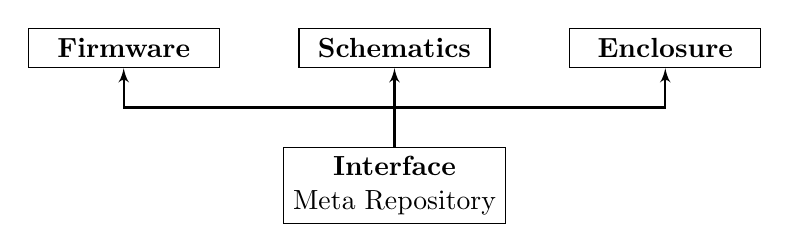
\begin{tikzpicture}[
      box/.style = {draw, minimum width=0.2\linewidth, minimum height=0.5cm, align=center},
      arrow/.style = {-latex', thick}
    ]
    
    % \node[box] (box1) {Firmware\\sub-module};
    % \node[box, right=of box1] (box2) {CAD\\sub-module};
    % \node[box, right=of box2] (box3) {Model Data\\sub-module};
    % \node[box, below=2cm of box2] (bottom) {Interface\\meta-repository};

    \node[box] (box1) {\textbf{Firmware}};
    \node[box, right=of box1] (box2) {\textbf{Schematics}};
    \node[box, right=of box2] (box3) {\textbf{Enclosure}};
    \node[box, below=1cm of box2] (bottom) {\textbf{Interface}\\Meta Repository};
    
    \draw[arrow] (bottom.north) -- ++(0,0.5) -| (box1.south);
    \draw[arrow] (bottom.north) -- ++(0,0.5) -| (box2.south);
    \draw[arrow] (bottom.north) -- ++(0,0.5) -| (box3.south);
    
    \end{tikzpicture}
    \caption{The DMI is divided into three submodules each representing the firmware, electronics schematics and enlosure modelling data. These submodules are collected into a single repository that represents the interface.}
    \label{fig:repo-relation}
\end{figure}

\subsection{Archiving}

Archiving provides a means by which a work can be cited.

A DMI as a research product \cite{xxx} is an object that should be citable. The paper describes the object, it is not object itself and there are instances where citing the object is more applicable than citing the paper based around it.

Archiving should provide a DOI with which to cite. Repositories may also provide a recommended citation, but this should very much be looked upon as a bandage to a broken system and not a solution. The very helpful citation file format CFF provides a means to have a structure citation to software, but unhelpfully, integration with GitHub prompts the user to ``Cite this Repository'' \url{https://docs.github.com/en/repositories/managing-your-repositorys-settings-and-features/customizing-your-repository/about-citation-files} which, as already discussed, is something to be avoided.

Archiving exposed a few practical challenges. Zenodo’s GitHub integration does not yet handle meta-repositories, requiring separate DOIs for each submodule with cross-references \cite{zenodo_1036_2025}. Likewise, the future of CAD data is tied to software sustainability: the discontinuation of Autodesk EAGLE \cite{autodesk_eagle_2024} effectively freezes its XML format, though conversion to KiCad remains available \cite{kicad_eagle_2024}. These lessons emphasise that openness depends not only on licensing but also on the careful selection of formats and hosting infrastructure.

\begin{figure}
    \centering
    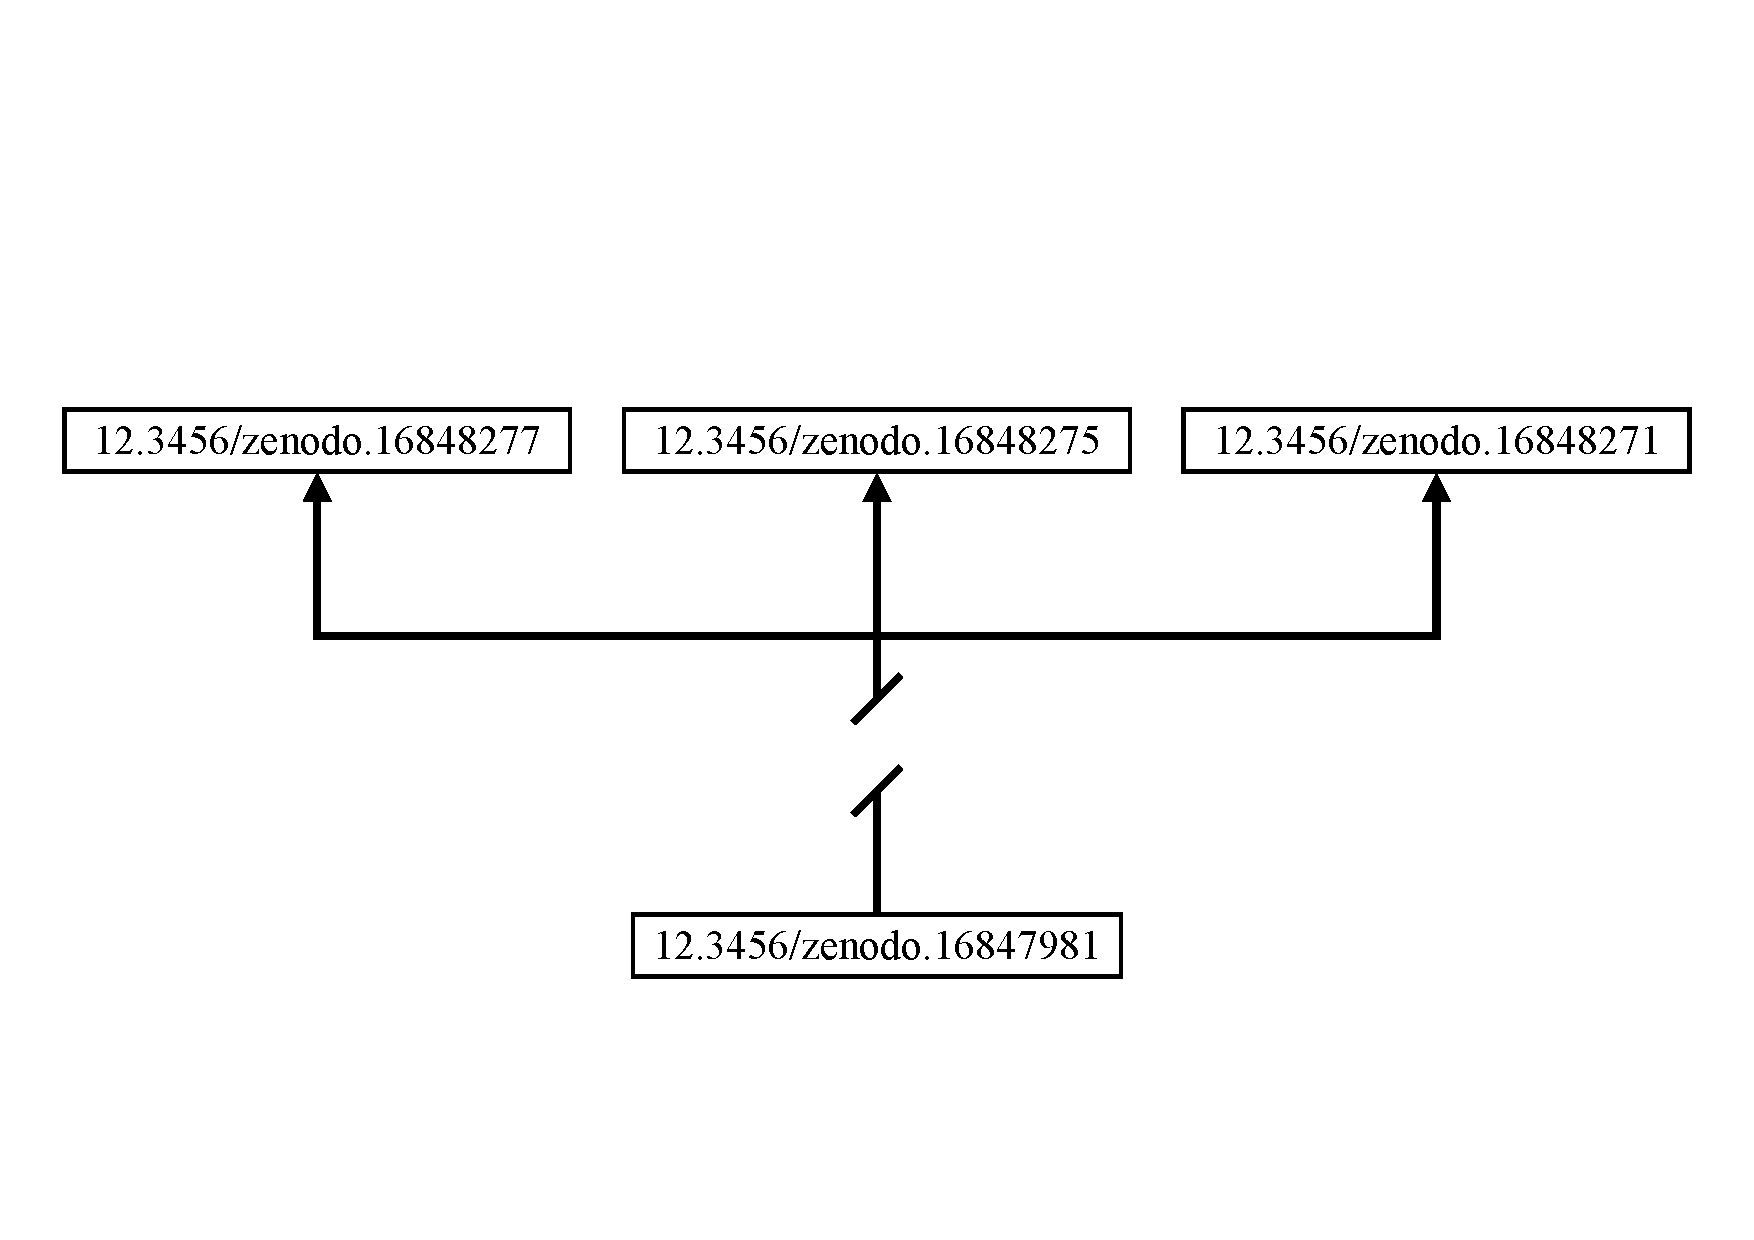
\includegraphics[width=1\linewidth]{images/modular_archive_1.pdf}
    \caption{Zenodo's GitHub integration does not include data in submodules. Alternative process is to archive each submodule at the relevant version and then archive the meta repository which contains the separate DOIs.}
    \label{fig:zenodo-github-integration}
\end{figure}

\subsubsection{limits in archiving modular projects}

Problem with a modular process is that zenodo's integration does not support it or a allow for easy configuration.

Would require the manual creation of the archive, copy the contents over. Alternatively, each submodule could be archived and a meta-archive simply contains reference to the constituent DOIs. This is not ideal but it is also not insurmaountable.



\subsection{Version Control $\neq$ Archiving}

a version control repository is not an archive.

longevity of a version control repository should be treated cautiously especially when it is privately owned. institutes could do more to provide these kind of services, but that is a separate discussion.

Version control allows a project to be explored in time. The version pertaining to the project should be tagged, of course, but a version control repository is a living document.

The content of a version control repository is alive and its location is ephemeral. A digital archive's content is static and location permanent.

Version control repository ideal for idea that iterate and where there is a desire to navigate a project's progression in time.

For citing work, given their static and permanent nature, archives and DOIs should be used.

\subsection{Documentation}

Following \citet{procida_diataxis_2025}, four complementary forms of
documentation can be distinguished: Tutorials, How-to guides, Explanation, and
Reference. These forms naturally divide into two audiences: user-facing and
developer-facing. Adapting \citet{procida_diataxis_2025}, developer-facing
documentation lies in the How-to and Reference categories, while user-facing
documentation is found in Tutorials and Explanation. This division is not
strict, as the binary of `user' and `developer' rarely holds true in practice;
rather, audiences exist along a continuum. Reference documentation can be
generated from source annotations to avoid duplication and support automation.
Across M\textsc{atlab}, Python, and C\textsc{++}, multiple conventions coexist
\cite{vanrossum_pep8_2001, goodger_pep257_2001}, supported by tooling ecosystems
such as Doxygen, Sphinx, and HeaderDoc.%
\footnote{See the Stack Overflow Data Explorer for indicative tag counts:
\url{https://data.stackexchange.com/stackoverflow/query/1069131/get-all-tags}.}
Even so, generated API references should not substitute for user manuals
\cite[Section~6.2]{stallman_gnu_1992}, though this is often the case
\cite{procida_diataxis_2025}.%
\footnote{\url{https://diataxis.fr/reference/}}

Best practice emphasises the importance of documentation
\cite{smith_software_2016}, though it is less prescriptive about form and depth.
\citet{writethedocs_sowftware_2025} offers comprehensive guidance; a
pragmatic rule is that documentation should enable you to still ``understand
your code in six months'' \cite{writethedocs_sowftware_2025}, a principle echoed
in reproducibility studies \cite{perkel_challenge_2020}. Using the
\citep{ssi_checklist_2018} checklist, the core requirements for an open research
software project are: publicly available source code, a version control system
(VCS), user and developer documentation, an OSI-compliant licence, and
persistent identifiers (typically DOIs). A public VCS implies source
availability, though the reverse is not guaranteed. Likewise, a DOI implies some
level of digital archiving, but a release archive does not necessitate a DOI.
DOIs should be assigned both to the software as a whole and to individual
releases \cite{smith_software_2016}; licences should be clearly stated and
OSI-compliant \cite{hong_choosing_2025}. To better support complex software
citation, \citet{druskat_citation_2021} introduced the Citation File Format
(CFF), which standardises metadata for software citations and is supported by
both GitHub and Zenodo. Recommendations in \citet{fiordelmondo_towards_2025}
extend this to hardware projects, with tools for citation
\cite{spaaks_cffconvert_2021}. Beyond these essentials (contribution policies,
issue tracking, codes of conduct), more advanced practices presuppose an active
repository.

Shallow submodules allow for only the relevant code for that commit to be pulled from the upstream repository meaning the full data weight of the entire repository is not needed.
Relevant for the ability to compartmentalise auto generated documentation which can be served from a sub-repository branch, but not clog up the  code base of the meta repository.
This was the case with the firmware \footnote{\url{https://nemus-project.github.io/harpsichord-interface-firmware/docs/html/}} for interface in \citet{hamilton_augmentation_2025_activities}.


\subsubsection{Software Documentation Practice}

The documentation practice for a project may also reveal something within the author's own perception of the work.
Documentation that leans heavily towards \textit{Reference} in the diataxis framework \citet{procida_diataxis_2025} are concerned with the technical understanding and modification of the work, something that is still in progress.
In the same framework, ``Tutorial'' documentation view the work is static, when the user's primary concern is with utilising the work. Through this lens we can assess a NIME and perhaps understand the intention for growth or reuse.

% \cite{burns_documents_2021}
% \begin{quote}
%     Case in point: I highly doubt anyone
% has learned to ride a bike by reading an instruction manual.
% \end{quote}
%  But somone needed to explain it


\section{Concluding Remarks}

Reluctance to share, anecdotally is that a work is `in-progress' which should be seen as a benefit. The appearance that work is in a highly finished polished state can be intimidating. the goal of NIME is should not always be to have a completed idea but to discuss ideas in progress. If that were the case we would \textit{only} be sharing pictures and archives, once something is finished, what isthere kef6t to discuss.

Designing Sensory NIME for Autism: ``Open-source development initiatives should be encouraged to foster 
scalability and inclusivity.''


Sharing with a wider community enables the possibility of research breaking out beyond the confines of its original life span. Enables the chance for more meaningful user evaluation \cite{calegario_documentation_2021} by reducing the barriers to accessing an interface. Ideas can be iterated upon, built upon previous work.

Source material varies from schematics to zine \cite{nime2025_42}.

% \citet{burns_documents_2021}
% \begin{quote}
%     Thus, even though the administration would agree
% that the library was a real place, it was only real to them as the “cobblestones” of the street are
% real—as opposed to whole streets with their social worlds and other components (the whole is
% reduced to a part that then becomes its perceived entire ontological substance; perhaps we can
% think of this as synecdochic fallacy38). However, per Polanyi, this is a failure to recognize
% emergence:
% This capacity of a thing to reveal itself in unexpected ways in the future I attribute to the
% fact that the thing observed is an aspect of a reality, possessing a significance that is not
% 14
% exhausted by our conception of any single aspect of it…. And since I regard the
% significance of a thing as more important than its tangibility, I shall say that minds and
% problems are more real than cobblestones.39
% If we can apply this lesson to the document, we could state that:
% Thesis 5: Tacit knowledge warns us against treating the digital document as if it is only a
% cobblestone.
% Yet this is what the open science movement does, not by introducing a new paradigm but
% by expanding the task assigned to the document—to document more, for example, under the
% FAIR principle (findable, accessible, interoperable, reusable).40
% \end{quote}

% Yet this is what the open science movement does, not by introducing a new paradigm but
% by expanding the task assigned to the document—to document more, for example, under the
% FAIR principle (findable, accessible, interoperable, reusable).40 
% Not to document more for the sake of documentation but to share and make open what is already there and what might already be being shared and open, but just done in a deliberate manner.
% work reduced to a cobblestone, be delibarate


% \subsection{Core principles}

% 1. It should be easy to find a repository (version control or archival)
% 2. if it exists, it should be in the paper
% 3. open should be the default
% 4.


\section{Recommendations}\label{sec:recommendations}

What the repository or archive of the DMI should contain has already been covered elsewhere, the specific contents are not fixed and will change from project to project

rather than focussing on a central repository \citet{mcpherson_nimehub_2016}, electing replicating officers \citet{calegario_documentation_2021} or conforming to standard format \citet{fiordelmondo_towards_2025} we can look at solution that are much simpler, but have a much wider impact

clear there is a desire to share work, offload the burden on choosing the most effective way to disseminate, or the reader in locating the work, the solution would be to standardise one, possibly two field that are in the papers template text, and in the metadata.

The burden to choose a format on the author and burden of finding it on the reader as opposed to an agreed format understood by both parties.


Table~\ref{tab:git_placement}
This is not a call to conform to this as standard practice, but the variation in placement shows there is no universal strategy by which the community has aligned. 
A suggested solution to address this is covered in section \ref{sec:recommendations}.


Section~\ref{sec:current-state}
In most cases there was a clear desire to make the work accessible, but with no clear format the link was overlooked.
Two repositories were private and subsequently made available, one repository had simply used the wrong link and alternate was provided.
For one repository, the authors were unreachable. Finally, one repository was found through a simple search. Including these papers which had intent, the total is 34 repositories.

\footnote{Or examples such as \textit{Embedded Comparo: Small DSP Systems Side-by-Side} where the git repository url is easily missed as a footnote hidden below references.}

The infrastructure exists \url{https://arxiv.org/} and \url{https://zenodo.org/} are openly available and relevant, withthe latter the standard archive for NIME proceedings.
\footnote{with the exception of 2022 and 2023 which use pubpub \url{https://nime.pubpub.org/previous-nimes}}
Part of the submission, the work can marked as closed source, if that is necessary but a mandatory field for project URL or DOI would curtail the open source agnosticism and make the choice a much more deliberate one.

NIME already provides a an entry in its metadata for an archive from which the paper's DOI is taken. Of the 96 NIME 2025 papers only 16 papers have supplementary files and these are exclusively videos.
When source material is extant and there is a clear intention on sharing it, it would appear that some barrier is present which prevents or dissuades authors from sharing their supplementary material.

\begin{figure}
    \centering
    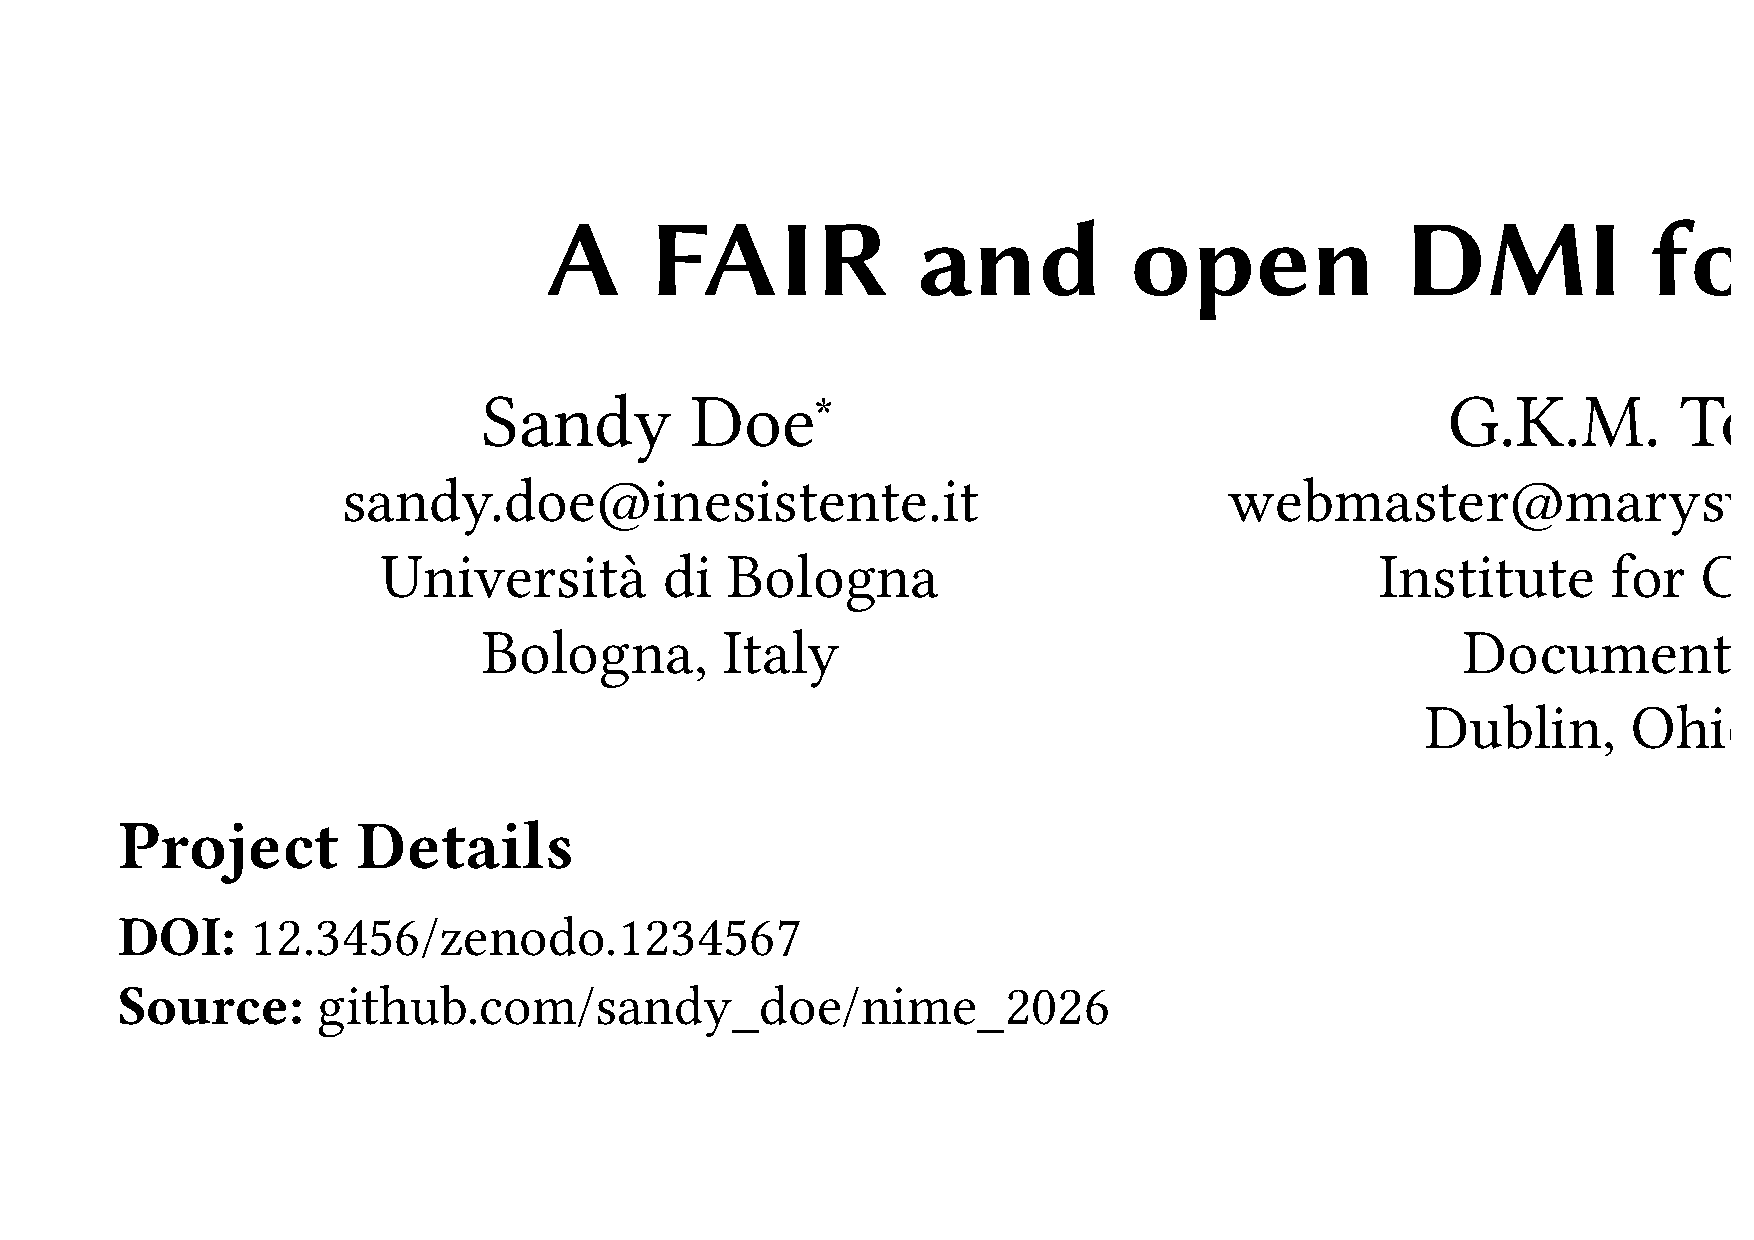
\includegraphics[width=\linewidth]{images/open-example.pdf}\\
    \vspace{0.5cm}
    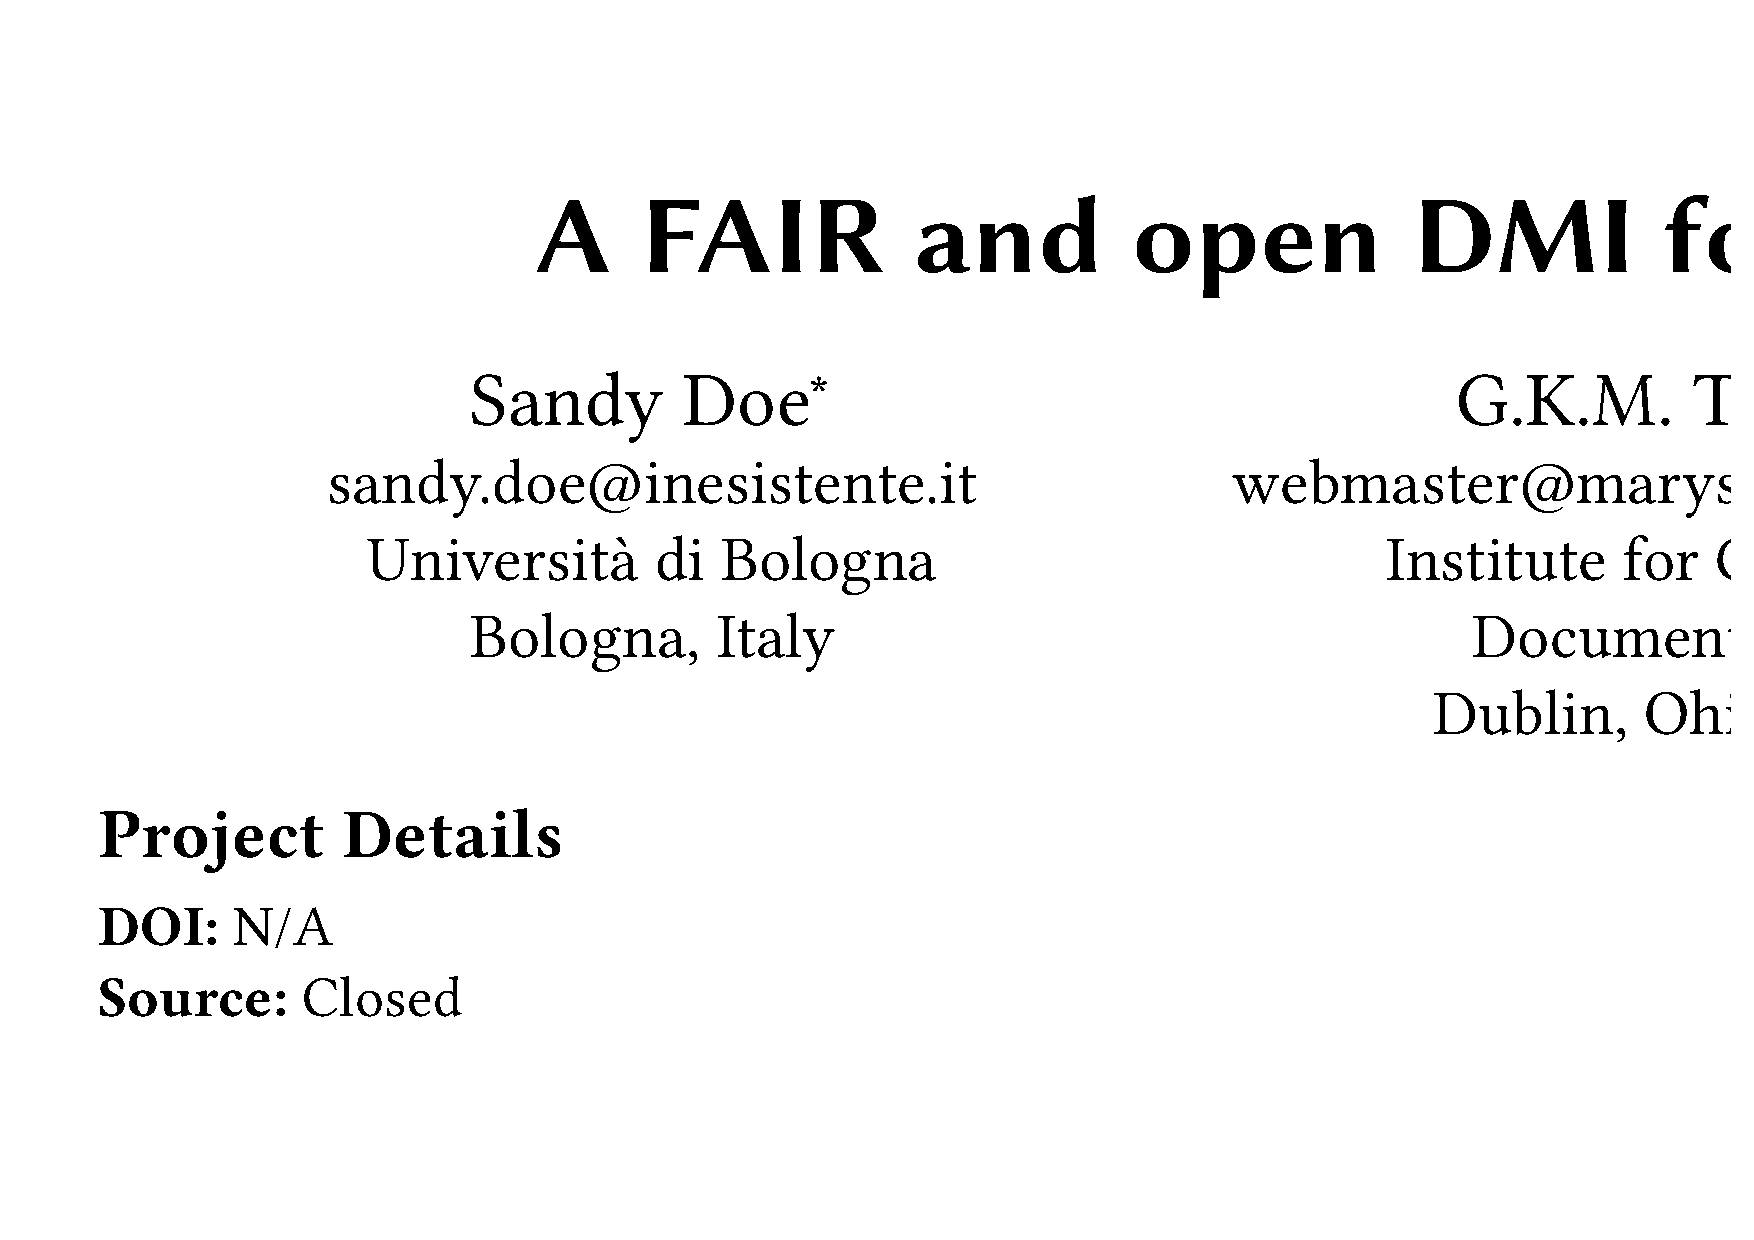
\includegraphics[width=\linewidth]{images/closed-example.pdf}    
    \caption{Project details as a standard field in the paper template, in the same manner of the title and authors, would allow for quick identification of the project status and files. These details are not obligatory and could be withheld, but the choice to do so becomes deliberate.}
    \label{fig:project-details}
\end{figure}

Aiming for some standardised template or central repository sets a high bar that the community is npt ready to meet. We may be missing even just the obvious solutions.
One can find the authors of a paper easily. Supplementary material in the form of a zenodo archive has a space on the NIME website, but it is clearly under utilised.

In the same way one can open a per and see immediately the title, authors, there should be a space for
a DOI to the source for which the material pertains or a notice in cases where the the work is either proprietary or the material has some other ethical restrictions.

For academic work, an open first approach should be the goal standard as recommended in the open science and FAIR principles. Closed by default because of a clear path to sign-post a repository is a huge waste.

for example: SMucK: Symbolic Music in ChucK is perfectly easy to find with a search, but it is missing any kind of link in the paper! (disqualified)

A standard metadata entry would ease future analysis.


fits in to the wider practice of citing digital research output, be it software, hardware, or data. The process very quickly becomes messy which is more often than not as the ideal is of a standard citation is not available.

This has been the case for this paper, and likely many papers at this years NIME.

% What is a clear order of precedence for citing sowftare?
A clear order of precedence

\begin{itemize}
\item DOI to the archive of the relevant version
\item SoftWare Hash IDentifier (SWHID) \cite{softwareheritage_archive_2025}
\item Citation File Format \cite{druskat_citation_2021}
\item Suggested citation format
\item Version-specific repository URL
\item General project URL
\end{itemize}

When citing software or data, precedence should favour a citation that prioritises longevity and version specificity over those that merely indicate location.

SoftWare Hash IDentifier (SWHID) ISO/IEC international standard 18670 on April 23, 2025.
Is passive, requires the repository be public and cannot guarantee that submodules have also been ingested. 

Like the web archive, this should be looked upon as a last ditch and a much more active and deliberate archiving approach should be taken

%% Sentiment: The intention is end on note that acknowledges that this isn't zero effort, but it is worth while. That nothing will improve if we do nothing. 
%% The sentiment is also that there is an implicit high bar and far to few are meeting it, so we should lower to an _explicit_. 
%% Perfect is the enemy of good, 
%% good-enough practice before best practice
The resistance is very much one of awareness and skill acquisition. Contributors are far more likely to follow the practice set out by there peers and their mentors. Change comes from above, and from the side and we should lead by example.

 % Word count - 200 words to cover the abstract


\section{Ethical Standards}
This study analyses publicly available NIME proceedings to identify references to project source material and their open source dependencies. Where repository links were unclear or missing, authors were contacted solely to clarify the location of publicly shared materials. No personal data beyond that already published in the proceedings was collected. The analysis focuses on infrastructural and archival practices rather than individual evaluation.

In line with the NIME Principles and Code of Practice on Ethical Research \cite{morreale_nime_2025}, care has been taken to treat published works respectfully and to avoid framing results in ways that single out individual authors or projects. Findings are reported at an aggregate level to support reflection on community practices while upholding values of fairness, transparency, and inclusivity.

\bibliographystyle{ACM-Reference-Format}
\bibliography{main}

\appendix

\section{Source Repository}
The scripts, data and \LaTeX created for this paper are available via the NEMUS organisation's public GitHub repository and its associated Zenodo archive \cite{this_paper}.

\end{document}
\endinput
%%
%% End of file `sample-nime-paper.tex'.
